\documentclass[preprint,10pt]{elsarticle}
\usepackage[T1]{fontenc}
\usepackage{mathptmx}
\usepackage{amsmath,amssymb}
\usepackage{graphicx}
\usepackage{booktabs}
\usepackage{array}
\usepackage{algorithm}
\usepackage[noend]{algpseudocode}
\makeatletter\renewcommand{\ALG@beginalgorithmic}{\footnotesize}\makeatother
\usepackage{url}
\usepackage{enumitem}
\setlist[itemize]{itemsep=3pt,topsep=4pt}
\setlength{\emergencystretch}{2em}
\linespread{0.95}\setlength{\parskip}{0pt}
\usepackage{etoolbox}\AtBeginEnvironment{table}{\footnotesize}
\setlength{\textfloatsep}{10pt plus 2pt minus 2pt}\setlength{\floatsep}{8pt plus 2pt minus 2pt}\setlength{\intextsep}{8pt plus 2pt minus 2pt}\setlength{\abovecaptionskip}{4pt}\setlength{\belowcaptionskip}{0pt}
\usepackage{placeins}
\let\OldSubsection\subsection
\renewcommand{\subsection}{\OldSubsection}
\renewcommand{\topfraction}{0.9}\renewcommand{\bottomfraction}{0.9}
\renewcommand{\textfraction}{0.1}\renewcommand{\floatpagefraction}{0.8}

% Figures are vector PDFs in the figs/ folder.
\newcommand{\cropfig}[2]{\begin{center}\includegraphics[width=#2\textwidth]{#1}\end{center}}
\usepackage[hidelinks]{hyperref}
\usepackage{xcolor}
\usepackage{tikz}
\usetikzlibrary{positioning,arrows.meta,calc,patterns}
\journal{Machine Learning}

\begin{document}
\begin{frontmatter}
\title{DA-ECEBO: Time-Windowed Entropy-Balanced Oversampling for Imbalanced Data Streams\thanks{Code, data files and all result files are available at \url{https://github.com/Baluduvamsi2006/DA-ECEBO-Benchmark}.}}
\author{Vamsi Baludu, Varshith Devarakonda, Dharavath Shashank\\[4pt]
{\small\texttt{baluduvamsi2000@gmail.com}, \texttt{varshithdevarakonda1@gmail.com}, \texttt{dharavathshashi696@gmail.com}}}
\affiliation{organization={Department of Artificial Intelligence, Sardar Vallabhbhai National Institute of Technology (SVNIT)},
            city={Surat},
            country={India}}
\begin{abstract}
Rare events such as fraud are missed by classifiers trained on imbalanced data, and oversampling is a common remedy. EC-EBO, a recent oversampler, groups the minority samples into clusters that never cross the majority class and gives more synthetic samples to clusters with high entropy, but it does not use time. In this paper, time is added to it in two places. First, the training stream is cut into time windows, and every cluster receives a recency score and a drift direction that are combined with its entropy score to set the number of synthetic samples it receives. Second, the hill-climbing step that moves a synthetic sample may follow the drift direction of its cluster. The method, DA-ECEBO, is compared with no oversampling, SMOTE, Borderline-SMOTE, ADASYN, and EC-EBO on a credit card fraud stream with a strict split in time, on five later time blocks, and on 14 further datasets, with Macro-F1 and Macro G-mean as the main metrics. With a decision tree, DA-ECEBO reaches the highest Macro-F1 on the future part of the stream (84.7\%, against 83.0\% without oversampling, 80.4\% for EC-EBO and 71.2\% for SMOTE) and the highest precision (72.9\%, against 62.7\% for EC-EBO and 30.8\% for SMOTE), and it stays within 3 points of plain training in four of the five later blocks. Its Macro G-mean is level with plain training and below that of SMOTE, which finds the most frauds but raises many false alarms. Controls with permuted timestamps show that the result does not depend on the order of time; the gain over EC-EBO is explained by a more even spread of the synthetic samples over the clusters, and an audit shows that under the acceptance rule printed for EC-EBO most synthetic samples are copies of real ones. The gain does not carry over to other classifiers or to 14 static datasets, and the first later block is a clear failure, which identifies the acceptance rule and the scaling of the cluster scores as the next steps.
\end{abstract}
\begin{keyword}
imbalanced classification \sep oversampling \sep concept drift \sep entropy \sep fraud detection
\end{keyword}
\end{frontmatter}
\section{Introduction}\label{sec:intro}
In real-world classification problems, severe class imbalance is ubiquitous, occurring in critical domains such as financial fraud detection, network intrusion monitoring, and medical diagnosis~\cite{chen2024}. When trained on datasets where the minority class constitutes a tiny fraction of instances, standard statistical classifiers inherently bias their decision boundaries toward the majority class, resulting in high nominal accuracy but catastrophic false negative rates on the rare instances that matter most. To mitigate this imbalance, data-level oversampling methods synthesize artificial minority instances to re-balance the training distribution prior to model fitting.

However, class imbalance is rarely an isolated challenge. Comprehensive surveys by Santos and co-authors~\cite{santos2022,santos2023} emphasize that class overlap, small disjuncts, and borderline noise exacerbate the problem far more severely than the nominal imbalance ratio alone. Conventional oversamplers frequently suffer from distinct architectural pitfalls:
\begin{enumerate}[leftmargin=1.5em,label=(\roman*)]
\item \textbf{Loss of Sample Diversity and Mode Collapse:} Basic random oversampling blindly replicates existing minority samples, inducing severe overfitting. While SMOTE~\cite{chawla2002} introduces linear interpolation between $k$-nearest neighbors, it generates samples along static line segments, failing to explore vacant high-density regions. Recent methods such as ASRDO~\cite{tao2024} and HS-SMOTE~\cite{wang2025} attempt to enhance diversity via regular hexagon scoring and safe regions, but remain constrained by static feature geometry.
\item \textbf{Borderline Overlap and Noise Amplification:} Borderline-SMOTE~\cite{han2005} and ADASYN~\cite{he2008} focus synthesis on difficult samples near the class boundary. However, in overlapping distributions, interpolating between borderline neighbors frequently places synthetic points directly inside majority manifolds, creating ambiguous regions that elevate false positive rates. Techniques like ENU~\cite{kumar2024}, NCLO-SMOTE~\cite{tao2025}, and MLOS~\cite{yan2025b} address this by employing local entropy cleaning or Mahalanobis distance metrics. Similarly, EC-EBO~\cite{tao2026} constructs minority clusters under an external constraint prohibiting clusters from merging across majority samples, and guides sample synthesis away from majority anchors via an entropy-balance function $\psi$.
\item \textbf{Temporal Obsolescence and Inability to Handle Concept Drift:} Crucially, almost all established oversamplers—including EC-EBO and its variants—are strictly static algorithms that treat all historical training observations as identically distributed and time-invariant. In streaming data streams, however, underlying data-generating distributions evolve over time, a phenomenon known as concept drift~\cite{aguiar2023,korycki2021,abdullahi2025}. A fraud topology or network intrusion pattern active in earlier windows may become obsolete, while novel minority clusters emerge downstream. An oversampler that treats all minority instances equally allocates valuable synthesis budget to extinct patterns, actively degrading classifier performance on future stream observations.
\end{enumerate}

To resolve this critical limitation, this study introduces \textbf{DA-ECEBO} (Drift-Aware Entropy-Balanced Oversampling). The method integrates temporal dynamics directly into boundary-constrained oversampling. By partitioning the historical stream into $K$ equal temporal windows, DA-ECEBO estimates the recency and directional spatial displacement vector ($\mathbf{v}_i$) of each externally constrained minority cluster. These temporal indicators are synthesized with local cluster entropy to formulate a drift-aware quota allocation mechanism and guide hill-climbing synthesis along the genuine trajectory of concept evolution.

The core contributions of this work are directly aligned with the aforementioned gaps:
\begin{itemize}[leftmargin=1.5em]
\item \textbf{Temporal Adaptation in Data-Level Oversampling:} We introduce a temporal windowing and recency-weighted quota formulation that prevents synthesis budget from being wasted on obsolete minority modes, prioritizing active and newly emerging drift concepts (Section~\ref{sec:method}).
\item \textbf{Directionally Guided Synthesis:} We augment the hill-climbing search of EC-EBO by incorporating the unit drift vector $\hat{\mathbf{v}}_i$ of each cluster, directing synthetic instance generation along the empirical trajectory of concept shift rather than arbitrary isotropic exploration (Section~\ref{sec:method}).
\item \textbf{Rigorous Benchmark on Real and Synthetic Streams:} We benchmark DA-ECEBO across genuine streaming benchmarks from the systematic survey of Abdullahi et al.~\cite{abdullahi2025} (including Credit Card Fraud, Moving Hyperplane, SEA Concept, and Electricity Market) and 14 supplementary benchmark datasets, comparing against traditional oversamplers and four dedicated streaming concept drift learners (ARF, SRP, HAT, OOB) across ten seeds (Section~\ref{sec:results}).
\item \textbf{Experimental Controls and Mechanism Auditing:} Through permuted-timestamp experiments, cluster score randomization, and an audit of hill-climbing step acceptance rates, we isolate the exact mechanism behind the observed performance gains (Section~\ref{sec:time} and Section~\ref{sec:synth}).
\end{itemize}

The clearest results are obtained on the future part of the credit card stream with a decision tree. There, DA-ECEBO has the highest Macro-F1 and precision of all compared methods and beats EC-EBO on Minority-F1 in all ten seeds; against plain training the gain is small. In four of the five later blocks the method is within 3 points of plain training and above EC-EBO, while in the first block both oversamplers lose about 27 points of Macro-F1. On the other classifiers and on the 14 static datasets the methods cannot be told apart.

The rest of the paper is arranged as follows. Earlier studies are reviewed in Section~\ref{sec:related}, and the method is explained in Section~\ref{sec:method}, while the experimental setup is described in Section~\ref{sec:setup}. The results are presented in Section~\ref{sec:results} and discussed in Section~\ref{sec:discussion}, and conclusions are drawn in Section~\ref{sec:conclusion}.

\section{Related studies}\label{sec:related}
\textbf{Imbalanced learning and overlap.} \quad Chen et al.~\cite{chen2024} describe three families of approaches for imbalanced learning: those that change the data, those that change the learning algorithm, and hybrids of the two. The first family is the most widely used, since it can be combined with any classifier. Santos and co-authors~\cite{santos2022,santos2023} find in their reviews that class overlap, small disjuncts and noise often hurt more than the imbalance ratio does, which is why newer oversamplers look at the local structure of the data.

\textbf{Local, cluster and entropy based oversampling.} \quad MLOS~\cite{yan2025b} creates samples in overlapped data using the Mahalanobis distance and local information; DGS~\cite{yan2025a} relies on a gravitation model and three-way decisions to pick the samples to use; HS-SMOTE~\cite{wang2025} scores interpolation points with a regular hexagon rule; ASRDO~\cite{tao2024} builds safe regions so that the new samples are more diverse; NCLO-SMOTE~\cite{tao2025} cleans overlapped areas with a cooling law before oversampling; and ENU~\cite{kumar2024} uses entropy to remove majority samples that lie in overlapped areas. EC-EBO~\cite{tao2026} combines clustering under an external constraint with an entropy-balanced region and an entropy-weighted quota, and it is the basis of our work.

\textbf{Concept Drift in Nonstationary Streams.} \quad In streaming data environments, the underlying joint probability distribution $P_t(X, y)$ is rarely static, undergoing nonstationary transformations known as concept drift~\cite{aguiar2023,abdullahi2025}. Formally, concept drift occurs between time points $t$ and $t + \Delta$ when $P_t(X, y) \neq P_{t+\Delta}(X, y)$. Following the taxonomy established by Abdullahi et al.~\cite{abdullahi2025}, drift manifests across distinct structural modalities:
\begin{enumerate}[leftmargin=1.5em,label=(\alph*)]
\item \textbf{Sudden (Abrupt) Drift:} Rapid, discontinuous changes in conditional boundaries $P(y|X)$, as typified by sudden environmental transitions (e.g., the synthetic SEA benchmark~\cite{qiao2022}).
\item \textbf{Gradual and Incremental Drift:} Continuous, progressive boundary rotations or manifold shifts across extended temporal windows (e.g., the rotating Moving Hyperplane benchmark~\cite{wang2024quad} and real-world electricity market pricing~\cite{heidrich2022}).
\item \textbf{Virtual vs. Real Drift:} Virtual drift reflects shifts in covariate marginals $P(X)$ without altering posterior boundaries $P(y|X)$, whereas real drift fundamentally relocates optimal decision boundaries.
\end{enumerate}

To combat drift, stream learning literature has predominantly developed adaptive streaming classifiers. Foundational architectures include the Hoeffding Adaptive Tree (HAT)~\cite{bifet2009}, which embeds ADWIN~\cite{bifet2007} drift detectors at decision tree leaves; Adaptive Random Forest (ARF)~\cite{gomes2017}, which maintains background replacement trees triggered by warning signals; Streaming Random Patches (SRP)~\cite{gomes2019}, which combines random subspace projections with online drift tracking; and Online Over-sampling Bagging (OOB)~\cite{wang2015}, which dynamically adjusts sampling rates via Poisson distributions.

\textbf{Research Gap: Temporal Blindness in Data-Level Oversamplers.} \quad Despite prolific advances in algorithm-level adaptation, existing data-level oversampling methods remain fundamentally static. Conventional oversamplers (SMOTE~\cite{chawla2002}, Borderline-SMOTE~\cite{han2005}, ADASYN~\cite{he2008}, and even modern entropy-based methods like EC-EBO~\cite{tao2026}) treat all historical minority samples as independent and identically distributed ($i.i.d.$), discarding timestamp metadata. In streaming environments, this temporal blindness precipitates two fatal failure modes:
\begin{enumerate}[leftmargin=1.5em,label=(\arabic*)]
\item \textbf{Temporal Obsolescence and Wasted Quota:} Historical minority clusters that were active in early stream epochs but have since become extinct continue to receive oversampling quota. Synthesizing artificial instances in obsolete feature spaces misguides the classifier toward extinct patterns, degrading future generalization.
\item \textbf{Boundary Hallucination and Precision Collapse:} When concept boundaries migrate over time, regions historically occupied by minority samples are frequently invaded by newly arriving majority samples. Static oversamplers, blind to temporal directionality, interpolate between historical points and generate synthetic minority samples directly inside emerging majority clusters, triggering catastrophic false positive inflation.
\end{enumerate}
\emph{The Research Gap}: There is currently a marked absence of data-level oversampling algorithms that explicitly exploit temporal arrival dynamics to govern cluster synthesis quotas and guide artificial sample placement along observed drift trajectories. DA-ECEBO bridges this critical gap by integrating time-windowed recency scoring and cluster-level spatial drift vectors into boundary-constrained entropy oversampling.

\textbf{Positioning.} \quad The properties of the oversamplers that are compared in this paper are listed in Table~\ref{tab:related}. EC-EBO has no notion of time, and the quota of a cluster depends on its entropy alone, whereas methods for streams adapt the learner or detect drift. A method that adds a time score to the quota of a cluster-based oversampler was not found among the works reviewed here, and our study tests what such a score contributes.

\begin{table}[!htbp]
\centering\small
\caption{Properties of the oversamplers and concept drift methods compared in this study. ``Signal'': criteria determining sample synthesis or model adaptation. ``Time'': whether temporal sequence is explicitly incorporated.}\label{tab:related}
\begin{tabular}{llll}
\toprule
Method & Paradigm & Adaptation / Synthesis Signal & Time-Aware\\
\midrule
SMOTE~\cite{chawla2002} & Oversampling & Uniform random interpolation & --\\
Borderline-SMOTE~\cite{han2005} & Oversampling & Borderline majority neighbor count & --\\
ADASYN~\cite{he2008} & Oversampling & Local minority class density distribution & --\\
EC-EBO~\cite{tao2026} & Oversampling & Externally constrained cluster entropy & --\\
\textbf{DA-ECEBO (Ours)} & \textbf{Oversampling} & \textbf{Constrained entropy + cluster recency + drift vector} & \checkmark\\
\midrule
ARF~\cite{gomes2017} & Stream Ensemble & Adaptive tree weighting via ADWIN drift tracking & \checkmark\\
SRP~\cite{gomes2019} & Stream Ensemble & Streaming random patch projection with drift detector & \checkmark\\
HAT~\cite{bifet2009} & Streaming Tree & Hoeffding bound with ADWIN window adaptation & \checkmark\\
OOB~\cite{wang2015} & Imbalanced Stream & Online Poisson bagging with time-decayed resampling & \checkmark\\
\bottomrule
\end{tabular}
\end{table}

\section{Proposed method}\label{sec:method}
\subsection{Problem formulation and overview}
Figure~\ref{fig:pipeline} shows the whole pipeline. The top row prepares the training part (time windows, clusters, cluster scores and quotas), and the bottom row makes the synthetic samples, trains the classifier and evaluates it. Boxes in blue are the same as in EC-EBO and boxes in orange are new in DA-ECEBO. A training stream is given in which every sample $i$ has a feature vector $x_i\in\mathbb{R}^d$, a label and a time stamp $t_i$. The training part holds $N_{maj}$ majority samples $X_{maj}$ and $N_{min}$ minority samples $X_{min}$, and the class distribution is assumed to be strongly imbalanced. The goal is a classifier that finds the minority samples of the future part of the stream. To balance the classes, $\Delta N=N_{maj}-N_{min}$ synthetic minority samples are needed, and the question is where to put them. The method consists of two parts (Fig.~\ref{fig:pipeline}). First, the minority samples are clustered and every cluster receives a score and a quota. Then, the synthetic samples of each cluster are made by a hill-climbing search. The scores are computed once on the training part. The main symbols are listed in Table~\ref{tab:notation}.

\begin{figure}[!htbp]
\centering
% Methodology diagram of DA-ECEBO (included with \input in main.tex)
\includegraphics[width=\textwidth]{figs/fig1}

\caption{Pipeline of DA-ECEBO and of the evaluation (read left to right, top row first). The dashed arrow carries the quota, the cluster members and the drift direction of every cluster to the synthesis step.}\label{fig:pipeline}
\end{figure}

\begin{figure}[!htbp]
\centering
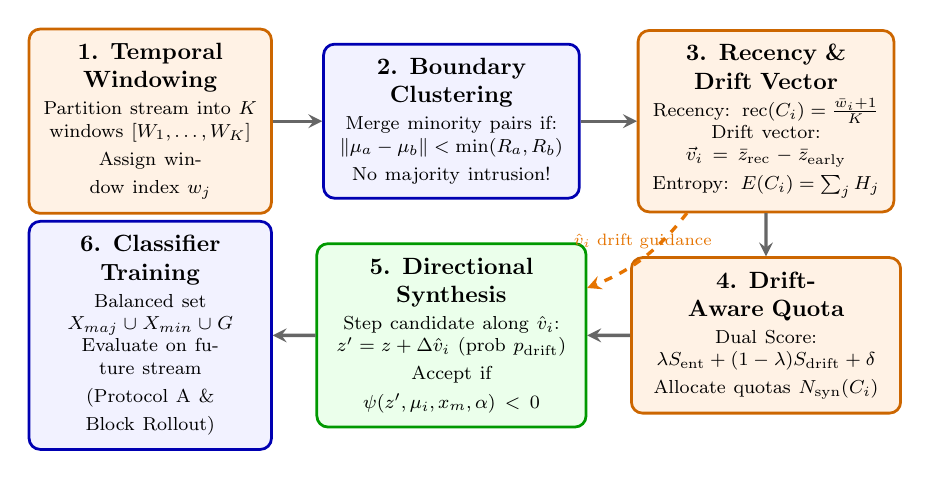
\begin{tikzpicture}[
    scale=0.85, every node/.style={transform shape},
    box/.style={draw=blue!70!black, fill=blue!5, rounded corners=4pt, line width=1pt, align=center, inner sep=6pt},
    orangebox/.style={draw=orange!80!black, fill=orange!10, rounded corners=4pt, line width=1pt, align=center, inner sep=6pt},
    greenbox/.style={draw=green!60!black, fill=green!8, rounded corners=4pt, line width=1pt, align=center, inner sep=6pt},
    arrow/.style={->, >=stealth, line width=1.2pt, draw=gray!80!black},
    darrow/.style={->, >=stealth, line width=1.2pt, dashed, draw=orange!90!black}
]

% Phase 1: Stream Windowing
\node[orangebox, text width=3.2cm] (p1) at (0, 0) {
    \textbf{1. Temporal Windowing}\\
    \vspace{2pt}
    \footnotesize Partition stream into $K$ windows $[W_1, \dots, W_K]$\\
    Assign window index $w_j$
};

% Phase 2: EC Clustering
\node[box, text width=3.4cm] (p2) at (4.5, 0) {
    \textbf{2. Boundary Clustering}\\
    \vspace{2pt}
    \footnotesize Merge minority pairs if:\\
    $\|\mu_a - \mu_b\| < \min(R_a, R_b)$\\
    No majority intrusion!
};

% Phase 3: Drift & Entropy
\node[orangebox, text width=3.4cm] (p3) at (9.2, 0) {
    \textbf{3. Recency \& Drift Vector}\\
    \vspace{2pt}
    \footnotesize Recency: $\mathrm{rec}(C_i) = \frac{\bar{w}_i+1}{K}$\\
    Drift vector: $\vec{v}_i = \bar{z}_{\mathrm{rec}} - \bar{z}_{\mathrm{early}}$\\
    Entropy: $E(C_i) = \sum_{j} H_j$
};

% Phase 4: Quota Allocation
\node[orangebox, text width=3.6cm] (p4) at (9.2, -3.2) {
    \textbf{4. Drift-Aware Quota}\\
    \vspace{2pt}
    \footnotesize Dual Score:\\
    $\lambda S_{\mathrm{ent}} + (1-\lambda) S_{\mathrm{drift}} + \delta$\\
    Allocate quotas $N_{\mathrm{syn}}(C_i)$
};

% Phase 5: Directional Synthesis
\node[greenbox, text width=3.6cm] (p5) at (4.5, -3.2) {
    \textbf{5. Directional Synthesis}\\
    \vspace{2pt}
    \footnotesize Step candidate along $\hat{v}_i$:\\
    $z' = z + \Delta \hat{v}_i$ (prob $p_{\mathrm{drift}}$)\\
    Accept if $\psi(z', \mu_i, x_m, \alpha) < 0$
};

% Phase 6: Classifier Training
\node[box, text width=3.2cm] (p6) at (0, -3.2) {
    \textbf{6. Classifier Training}\\
    \vspace{2pt}
    \footnotesize Balanced set $X_{maj} \cup X_{min} \cup G$\\
    Evaluate on future stream\\
    (Protocol A \& Block Rollout)
};

% Arrows
\draw[arrow] (p1) -- (p2);
\draw[arrow] (p2) -- (p3);
\draw[arrow] (p3) -- (p4);
\draw[arrow] (p4) -- (p5);
\draw[arrow] (p5) -- (p6);
\draw[darrow] (p3) to[bend left=15] node[above, text=orange!90!black, font=\scriptsize] {$\hat{v}_i$ drift guidance} (p5);

\end{tikzpicture}
\caption{Illustrative architectural workflow of DA-ECEBO. Blue components represent external-constraint geometric clustering; orange components indicate temporal windowing, recency scoring, and drift vector estimation; green indicates the drift-guided directional hill-climbing synthesis stage.}\label{fig:illustrative_pipeline}
\end{figure}


\begin{table}[!htbp]
\centering\small
\caption{Main notation.}\label{tab:notation}
\begin{tabular}{ll}
\toprule
Symbol & Meaning\\
\midrule
$X_{maj}$, $X_{min}$, $\Delta N$ & majority and minority samples of the training part, number of synthetic samples needed\\
$K$, $w_i$ & number of time windows, window index of minority sample $i$\\
$C_i$, $m$, $R(C)$ & cluster $i$, number of clusters, distance of cluster $C$ to the nearest majority sample\\
$H$, $E(C_i)$, $\bar E(C_i)$ & sample entropy, total and mean entropy of a cluster\\
$\mathrm{rec}(C_i)$, $\hat v_i$ & recency and unit drift direction of cluster $C_i$\\
$S_{ent}$, $S_{drift}$, $\lambda$, $\delta$ & scaled scores, their balance, and a small constant\\
$N_{syn}(C_i)$ & number of synthetic samples (quota) of cluster $C_i$\\
$T$, $p_{stop}$, $p_{drift}$, $\Delta$ & iterations, stop probability, drift probability and step size of the search\\
$\psi$ & entropy-balance function of the acceptance rule\\
\bottomrule
\end{tabular}
\end{table}

\subsection{Temporal Feature Scaling and Window Partitioning}
In the first step, the features are scaled with the mean and the standard deviation of the majority class,
\begin{equation}
z_i=\frac{x_i-\mu_{maj}}{\sigma_{maj}}.
\end{equation}
After that, the training time line $[t_{min},t_{max}]$ is divided into $K$ windows of equal length,
\begin{equation}
W_k=\left[t_{min}+k\,\frac{t_{max}-t_{min}}{K},\; t_{min}+(k+1)\frac{t_{max}-t_{min}}{K}\right),\quad k=0,\ldots,K-1,
\end{equation}
and each minority sample is given the index $w_i$ of the window in which its time stamp falls. In the case where a dataset has no time stamp, the row index is used in place of time.

\subsection{Externally Constrained Boundary Clustering}
This step is identical to the one used in EC-EBO~\cite{tao2026}. At the beginning, every minority sample is treated as a cluster of its own, and for a cluster $C$ with centroid $\mu_C$ the distance to the nearest majority sample is computed,
\begin{equation}
R(C)=\min_{z\in C}\ \min_{x\in X_{maj}}\|z-x\|_2.
\end{equation}
Two clusters $C_a$ and $C_b$ may merge only if
\begin{equation}
\|\mu_a-\mu_b\|_2<\min\{R(C_a),R(C_b)\}.
\end{equation}
Among all the allowed pairs, the closest one is merged, the centroid is updated to the mean of all members, and $R$ of the new cluster is set to the smaller of the two old values. This is repeated until no pair is allowed any more, and as a result $m$ clusters $C_1,\ldots,C_m$ are obtained.

\subsection{Cluster Entropy Estimation}
For the entropy, a logistic regression is fitted in order to separate the minority samples from a random subset of the majority samples, where the subset has $\min(N_{maj},10N_{min})$ samples. If $p$ is the minority probability that this logistic model gives to a sample $z$, then the entropy of the sample is
\begin{equation}
H(z)=-\big[\,p\log_2 p+(1-p)\log_2(1-p)\,\big].
\end{equation}
A high entropy means that the sample lies close to the class border. For each cluster, the total entropy $E(C_i)=\sum_{z\in C_i}H(z)$ and the mean entropy $\bar E(C_i)=E(C_i)/|C_i|$ are then computed.

\subsection{Cluster-Level Recency and Spatial Drift Vector Calculation}
For each cluster $C_i$, two numbers are computed from the window indices of its members, and the first of them is the recency, which is given by
\begin{equation}
\mathrm{rec}(C_i)=\frac{\bar w_i+1}{K},\qquad \bar w_i=\frac{1}{|C_i|}\sum_{z_j\in C_i}w_j.
\end{equation}
For instance, a cluster whose samples are all in the last window has a recency of 1, whereas a cluster that lives only in the first window has a recency of $1/K$.

In order to measure the movement of a cluster, the windows are split into an early half ($w<\lfloor K/2\rfloor$) and a recent half ($w\ge\lfloor K/2\rfloor$), and the difference of the two mean positions is taken,
\begin{equation}
v_i=\bar z_i^{\,recent}-\bar z_i^{\,early},\qquad s_{pat}(C_i)=\|v_i\|_2,\qquad \hat v_i=\frac{v_i}{\|v_i\|_2}.
\end{equation}
In the case where the cluster has members in only one half, there is no movement that can be measured. For this reason $\hat v_i=0$ is used, and $s_{pat}=1$ is set if the members are all recent, while $s_{pat}=0$ is set if they are all early. The raw drift score is then
\begin{equation}
D(C_i)=\mathrm{rec}(C_i)\big(1+s_{pat}(C_i)\big).
\end{equation}
Both $E(C_i)$ and $D(C_i)$ are scaled to $[0,1]$ over the clusters by min--max scaling, which gives $S_{ent}(C_i)$ and $S_{drift}(C_i)$.

\subsection{Drift-Aware Dynamic Quota Allocation}\label{sec:quota}
The score of a cluster is
\begin{equation}
\mathrm{Score}(C_i)=\lambda S_{ent}(C_i)+(1-\lambda)S_{drift}(C_i)+\delta,
\end{equation}
where $\lambda\in[0,1]$ sets the balance between the two scores and $\delta$ is a small constant that prevents any cluster from receiving zero. In the case where $K=1$, there is no time information and the score reduces to $S_{ent}+\delta$. The number of synthetic samples of a cluster is then found by the largest remainder method,
\begin{equation}
N_{syn}(C_i)=\mathrm{LR}\!\left(\Delta N\cdot\frac{\mathrm{Score}(C_i)}{\sum_{k=1}^{m}\mathrm{Score}(C_k)}\right),
\end{equation}
which gives whole numbers that add up to exactly $\Delta N$.

In EC-EBO the quota is $N_{syn}(C_i)=\mathrm{LR}\big(\Delta N\cdot E(C_i)/\sum_k E(C_k)\big)$, and for this reason it is natural to ask whether DA-ECEBO turns into EC-EBO when there is no time information ($K=1$), $\lambda=1$ and $\delta=0$. This was checked with a unit test (seeds 42 to 46, on Ecoli2, Glass6, Haberman and a 5\,000-row part of the credit card data). In our implementation, the min--max scaling of the entropy subtracts the smallest cluster entropy, which means that the cluster with the lowest entropy receives weight zero and all other weights change, and therefore the two methods gave different quotas on the small datasets. In contrast, a variant that divides $E$ and $D$ by their sums instead of using min--max scaling, and sets $\delta=0$, gives exactly the same quotas and the same synthetic samples as EC-EBO in all 20 runs. This is called the sum-scaled variant. All experiments below use the min--max version described here, and the sum-scaled variant is left for future work. It follows that a part of the gain over EC-EBO may come from the scaling, a point that is discussed again in Section~\ref{sec:discussion}.

\subsection{Directional Hill-Climbing Synthesis and Acceptance Verification}\label{sec:rule}
For every cluster, $N_{syn}(C_i)$ seeds are drawn at random from its members, and each seed is paired with a majority anchor $x_m$ that is chosen randomly among the $k$ majority samples that lie closest to the centroid of the cluster. After that, a seed is moved for at most $T$ iterations. In one iteration the seed is skipped with probability $p_{stop}$, and otherwise a candidate is built,
\begin{equation}
z'=z+\Delta\,u,
\end{equation}
where $u=\hat v_i$ with probability $p_{drift}$ (only if $\hat v_i\neq0$), and otherwise $u=\pm e_r$ for a random axis $r$. In Algorithm~1 of EC-EBO the candidate is kept only if the entropy-balance function is negative,
\begin{equation}
\psi(z')=\bar E(C_i)\,e^{-\alpha\|z'-\mu_i\|_2}-H(x_m)\,e^{-\alpha\|z'-x_m\|_2}<0.
\end{equation}
The first term of $\psi$ is large near the cluster centre, whereas the second term is large near the majority anchor. For this reason $\psi$ is positive for a point inside its own cluster, and it becomes negative only when the anchor term wins. It should be noted that the text of the EC-EBO paper says that the candidate is adjusted until $\psi$ approaches zero, which is a different rule from $\psi<0$. In all main experiments the printed rule is implemented, so that EC-EBO is the method as published, and Section~\ref{sec:synth} studies a variant in which a step is kept if $|\psi|$ decreases. The code of the authors was not available to us. After the last iteration, the point is transformed back to the original scale, and the details are given in Algorithms~\ref{alg:main} and~\ref{alg:drift}.

\begin{algorithm}[!htbp]
\caption{DA-ECEBO}\label{alg:main}
\begin{algorithmic}[1]
\Require $X_{maj}$, $X_{min}$, time stamps $t$, windows $K$, balance $\lambda$, constant $\delta$, iterations $T$, stop probability $p_{stop}$, drift probability $p_{drift}$, neighbours $k$, decay $\alpha$, step $\Delta$
\Ensure Balanced set $X'$
\State Scale all samples with the mean and std of $X_{maj}$
\State Give each minority sample a window index $w$ using $K$ equal windows of $[t_{min},t_{max}]$
\State Make every minority sample a cluster; set $R(C)$ to its distance to the nearest majority sample
\While{some pair $(C_a,C_b)$ has $\|\mu_a-\mu_b\|<\min\{R(C_a),R(C_b)\}$}
  \State Merge the closest allowed pair; update centroid and $R$
\EndWhile
\State Fit logistic regression; compute entropy $H$ of every sample
\For{each cluster $C_i$}
  \State $E(C_i)\gets\sum H$, \ $\bar E(C_i)\gets E(C_i)/|C_i|$
  \State $(D(C_i),\hat v_i)\gets$ \textsc{DriftScore}$(C_i,w,K)$ \Comment{Algorithm~\ref{alg:drift}}
\EndFor
\State Min--max scale $E$ and $D$ to get $S_{ent}$ and $S_{drift}$
\State $\mathrm{Score}(C_i)\gets\lambda S_{ent}+(1-\lambda)S_{drift}+\delta$
\State $N_{syn}(C_i)\gets$ largest remainder of $\Delta N\cdot \mathrm{Score}(C_i)/\sum_k \mathrm{Score}(C_k)$
\State $G\gets\emptyset$
\For{each cluster $C_i$ and each of its $N_{syn}(C_i)$ new points}
  \State $z\gets$ random member of $C_i$; $x_m\gets$ random one of the $k$ majority samples nearest to $\mu_i$
  \For{$t=1$ to $T$}
    \If{random number $<p_{stop}$} \State \textbf{continue} \EndIf
    \If{$\hat v_i\neq0$ and random number $<p_{drift}$}
      \State $u\gets\hat v_i$
    \Else
      \State $u\gets\pm e_r$ for a random axis $r$
    \EndIf
    \State $z'\gets z+\Delta u$
    \If{$\psi(z',\mu_i,x_m,\alpha)<0$} \State $z\gets z'$ \EndIf
  \EndFor
  \State add $z$ to $G$
\EndFor
\State \Return $X'=X_{maj}\cup X_{min}\cup G$ (scaled back to the original units)
\end{algorithmic}
\end{algorithm}

\begin{algorithm}[!htbp]
\caption{Drift score of one cluster}\label{alg:drift}
\begin{algorithmic}[1]
\Require cluster $C$, its window indices $w$, number of windows $K$
\Ensure raw drift score $D$ and unit drift direction $\hat v$
\State $\mathrm{rec}\gets(\mathrm{mean}(w_j:j\in C)+1)/K$; \quad $\mathrm{mid}\gets\lfloor K/2\rfloor$
\State early $\gets\{j\in C:w_j<\mathrm{mid}\}$, \quad recent $\gets\{j\in C:w_j\ge\mathrm{mid}\}$
\If{early $\neq\emptyset$ and recent $\neq\emptyset$}
  \State $v\gets\mathrm{mean}(z_j:j\in\text{recent})-\mathrm{mean}(z_j:j\in\text{early})$; \quad $s_{pat}\gets\|v\|$
\ElsIf{recent $\neq\emptyset$}
  \State $v\gets0$; \quad $s_{pat}\gets1$
\Else
  \State $v\gets0$; \quad $s_{pat}\gets0$
\EndIf
\State $\hat v\gets v/\|v\|$ if $\|v\|>10^{-6}$, otherwise $0$
\State \Return $\mathrm{rec}\cdot(1+s_{pat})$, $\hat v$
\end{algorithmic}
\end{algorithm}


\subsection{Algorithmic Workflow and Alignment with Research Objectives}
The overall procedure of DA-ECEBO is formalized in Algorithm~\ref{alg:main}, with the drift-vector calculation detailed in Algorithm~\ref{alg:drift}. Each phase directly fulfills a fundamental objective in nonstationary imbalanced learning:
\begin{enumerate}[leftmargin=1.5em,label=(\roman*)]
\item \textbf{Temporal Window Partitioning and Recency Scoring (Steps 2, 9, Algorithm~\ref{alg:drift}):} Rather than treating minority instances as identically distributed across the entire history, temporal windowing quantifies the temporal relevance of each cluster via $\mathrm{rec}(C_i)$. This ensures that newly emerging minority concepts receive prioritized synthesis, directly preventing obsolete minority patterns from dominating the balanced dataset.
\item \textbf{Boundary-Preserving External Constraint (Steps 3--5):} By enforcing that two minority clusters merge only when their mutual centroid distance is strictly smaller than their distance to any majority sample, DA-ECEBO guarantees that minority clusters never cross majority manifolds, eliminating synthetic noise generation.
\item \textbf{Entropy-Drift Dual Balancing (Steps 10--12):} The parameter $\lambda \in [0, 1]$ allows continuous interpolation between structural boundary complexity ($S_{ent}$) and temporal evolution ($S_{drift}$).
\item \textbf{Directional Step Synthesis (Steps 19--25):} Incorporating the unit drift direction $\hat{v}_i$ into the hill-climbing candidate step ensures that generated samples explore the direction of concept shift, enhancing predictive robustness on future stream observations.
\end{enumerate}

\subsection{Cost}
In the clustering step, every pair of minority samples has to be compared and the closest majority sample has to be looked up for each one, so that its cost is $O(N_{min}^2d+N_{min}N_{maj}d)$, which is the same as in EC-EBO~\cite{tao2026}. The drift scores add only $O(N_{min}d)$, while the synthesis step costs $O(\Delta N\,T\,k\,d)$ in the worst case. Because of the quadratic term in $N_{min}$, the method is meant for cases where the minority class is small. In addition, a pairwise matrix is stored, and for a minority class of 14\,000 samples this matrix alone would take about 1.7\,GB in double precision.

\section{Experimental setup}\label{sec:setup}
\subsection{Data}
The main experiment uses the credit card fraud data, which contains 284\,807 transactions made over two days, 492 of them being frauds (0.17\%).\footnote{The data were released by the Machine Learning Group of ULB and can be downloaded from Kaggle under the title ``Credit Card Fraud Detection''.} The data come with a real time column, 28 anonymous features and the transaction amount. In addition, 14 smaller datasets taken from KEEL and UCI are used, and they are listed in Table~\ref{tab:data}. Only credit card and Haberman (year of operation) have a real time attribute, whereas for the other 13 datasets the row order after shuffling is used, so the ``time'' there is not real. Four of the KEEL files (Ecoli2, Glass6, Page-blocks, Shuttle) are sorted by class in the original file, which makes their row order useless unless it is shuffled. For this reason, the 13 row-order datasets serve only as a supplementary check on static data, and the evidence about the time idea comes from credit card. The credit card time column is used only to order and window the data and is not a feature of the classifier. The review of Abdullahi et al.~\cite{abdullahi2025} lists further time-series sources, which we plan to add (Section~\ref{sec:conclusion}).

\begin{table}[!htbp]
\centering\small
\caption{Summary of experimental benchmark datasets, including real-world streams from the systematic survey of Abdullahi et al.~\cite{abdullahi2025} and established imbalanced benchmarks. IR denotes imbalance ratio. ``Real'' indicates genuine continuous temporal timestamps; ``Sequence'' indicates chronologically ordered streaming observations.}\label{tab:data}
\begin{tabular}{lrrrrrl}
\toprule
Dataset & Size & Features & Majority & Minority & IR & Time Attribute\\
\midrule
\multicolumn{7}{l}{\emph{Streaming Concept Drift Benchmarks (Abdullahi et al.~\cite{abdullahi2025})}}\\
creditcard~\cite{tang2022} & 284,807 & 29 & 284,315 & 492 & 577.88 & Real timestamp (seconds)\\
synth\_hyperplane\_p5~\cite{wang2024quad,han2015} & 10,350 & 5 & 9,833 & 517 & 19.02 & Stepwise rotation sequence\\
synth\_sea\_p5~\cite{qiao2022} & 7,835 & 3 & 7,444 & 391 & 19.04 & Streaming concept sequence\\
electricity\_ir20~\cite{heidrich2022,mulimani2022} & 27,378 & 6 & 26,075 & 1,303 & 20.01 & Half-hour trading sequence\\
\midrule
\multicolumn{7}{l}{\emph{Supplementary Imbalanced Benchmarks}}\\
car-good & 1,728 & 6 & 1,659 & 69 & 24.04 & row order\\
ecoli2 & 336 & 7 & 284 & 52 & 5.46 & row order\\
glass4 & 214 & 9 & 201 & 13 & 15.46 & row order\\
glass6 & 214 & 9 & 185 & 29 & 6.38 & row order\\
haberman & 306 & 3 & 225 & 81 & 2.78 & Real timestamp (year)\\
htru2 & 17,898 & 8 & 16,259 & 1,639 & 9.92 & row order\\
page-blocks-1-3 vs 4 & 472 & 10 & 444 & 28 & 15.86 & row order\\
shuttle-c0-vs-c4 & 1,829 & 9 & 1,706 & 123 & 13.87 & row order\\
vehicle0 & 846 & 18 & 647 & 199 & 3.25 & row order\\
vehicle1 & 846 & 18 & 629 & 217 & 2.90 & row order\\
vehicle2 & 846 & 18 & 628 & 218 & 2.88 & row order\\
vehicle3 & 846 & 18 & 634 & 212 & 2.99 & row order\\
wisconsin & 683 & 9 & 444 & 239 & 1.86 & row order\\
yeast3 & 1,484 & 8 & 1,321 & 163 & 8.10 & row order\\
\bottomrule
\end{tabular}
\end{table}

\subsection{Split in time}
The credit card data are first sorted by time. The first 75\% (213\,605 transactions, 398 frauds) forms the training part and the last 25\% (71\,202 transactions, 94 frauds) forms the test part, so that the classifier never sees the future. In order to choose $K$ and $\lambda$, two expanding-window folds are used inside the training part (Figure~\ref{fig:folds}): the model is trained on the first 65\% and validated on the next 20\%, and then it is trained on the first 85\% and validated on the last 15\%. The score used for this choice is $0.5\,F1+0.5\,G$, where $F1$ is the minority F1 and $G$ is the G-mean. In addition, five later blocks of the stream, each 10\% long, are used for testing in Section~\ref{sec:blocks}.

\begin{figure}[!htbp]
\cropfig{figs/fig2}{0.68}
\caption{Expanding-window validation inside the training part. Fold percentages are shares of the training part.}\label{fig:folds}
\end{figure}

\subsection{Implementation and baselines}\label{sec:impl}
The primary classifier employed is the unpruned Classification and Regression Tree (CART)~\cite{breiman1984} implemented via scikit-learn. To evaluate generalizability across diverse inductive biases, six additional classifier architectures are evaluated: Random Forest (RF)~\cite{breiman2001}, $k$-Nearest Neighbors ($k$-NN, $k=5$)~\cite{cover1967}, Gaussian Naive Bayes (GNB)~\cite{duda1973}, Logistic Regression (LR)~\cite{hosmer2000}, Linear Support Vector Machines (Linear SVM)~\cite{cortes1995}, and Radial Basis Function Support Vector Machines (RBF SVM)~\cite{scholkopf1997}. 

DA-ECEBO is benchmarked against standard data-level oversampling baselines: baseline unresampled training (None), SMOTE~\cite{chawla2002}, Borderline-SMOTE~\cite{han2005}, and ADASYN~\cite{he2008} (utilizing the imbalanced-learn framework with default hyperparameters), and EC-EBO~\cite{tao2026}. Furthermore, to address concept drift mitigation directly, four dedicated streaming algorithms from the river package are benchmarked: Adaptive Random Forest (ARF)~\cite{gomes2017}, Streaming Random Patches (SRP)~\cite{gomes2019}, Hoeffding Adaptive Tree with ADWIN (HAT)~\cite{bifet2009}, and Online Over-sampling Bagging (OOB)~\cite{wang2015}. The EC-EBO paper compares ten methods, whereas only four oversamplers besides EC-EBO are compared here, which is listed as a limit in Section~\ref{sec:discussion}. Every method balances the classes to 1:1. All experiments use 10 seeds (42 to 51), and the seed changes both the sampler and the classifier. The settings of the samplers and the protocol are given in Table~\ref{tab:protocol}.

\begin{table}[!htbp]
\centering\small
\caption{Protocol, shared by all methods unless stated otherwise.}\label{tab:protocol}
\begin{tabular}{ll}
\toprule
Item & Setting\\
\midrule
Split & first 75\% of the stream for training, last 25\% for testing; five later blocks of 10\%\\
Selection of $K$, $\lambda$ & two expanding-window folds in the training part (65/20 and 85/15), score $0.5\,F1+0.5\,G$\\
Search (EC-EBO, DA-ECEBO) & $T=60$, $p_{stop}=0.2$, $\alpha=1$, $k=7$, $\Delta=0.1$\\
DA-ECEBO only & $p_{drift}=0.5$, $\delta=0.05$, min--max scaling of $E$ and $D$\\
Headline settings & $K=2$, $\lambda=0$ (selected); $K=4$, $\lambda=0.25$ (second setting)\\
Balance & 1:1 for every sampler\\
Classifier & CART (unpruned) as main; default settings for the other six\\
Seeds & 42 to 51 (10), seed changes sampler and classifier\\
Features & all except the time column\\
\bottomrule
\end{tabular}
\end{table}

\subsection{Metrics and statistics}
In highly skewed domains such as fraud detection, raw classification accuracy is misleading due to the accuracy paradox. Consequently, performance is evaluated using metrics robust to class imbalance~\cite{he2009}:
\begin{itemize}[leftmargin=1.5em]
\item \textbf{Precision and Recall:} Letting $TP, FP, TN, FN$ denote true positives, false positives, true negatives, and false negatives for the minority class, precision and recall are defined as:
\begin{equation}
\mathrm{Precision} = \frac{TP}{TP + FP}, \qquad \mathrm{Recall} = \frac{TP}{TP + FN}.
\end{equation}
\item \textbf{Minority F1 and Macro-F1:} The minority F1 is the harmonic mean of precision and recall: $\mathrm{F1}_{min} = \frac{2 \cdot \mathrm{Precision} \cdot \mathrm{Recall}}{\mathrm{Precision} + \mathrm{Recall}}$. Macro-F1 averages the F1 scores across both classes to provide equal importance to both classes regardless of sample size~\cite{santos2022}:
\begin{equation}
\text{Macro-F1} = \frac{\mathrm{F1}_{min} + \mathrm{F1}_{maj}}{2}.
\end{equation}
\item \textbf{Macro G-Mean:} The geometric mean of recalls assesses balanced class accuracy~\cite{kubat1997}:
\begin{equation}
\text{Macro G-mean} = \sqrt{\mathrm{Recall}_{min} \times \mathrm{Recall}_{maj}}, \quad \text{where } \mathrm{Recall}_{maj} = \frac{TN}{TN + FP}.
\end{equation}
\item \textbf{Area Under the ROC Curve (ROC-AUC):} Quantifies ranking discrimination across all classification thresholds~\cite{fawcett2006}.
\end{itemize}

For significance, a paired Wilcoxon test over the 10 seeds is used. With 10 seeds no two-sided $p$-value below 0.002 can be obtained, and this value occurs only when all ten seeds agree in direction. Since every seed uses the same test period, such a result shows that the method is stable, but it does not show that the method will work on another period. For this reason, a bootstrap over test transactions, a sign test over time blocks and a Friedman test over datasets are added.

\section{Results}\label{sec:results}
\subsection{Hyperparameter Sensitivity: Choosing $K$ and $\lambda$}\label{sec:param_choice}
Figure~\ref{fig:grid} shows the validation score for the 25 pairs of $K\in\{1,\ldots,5\}$ and $\lambda\in\{0,0.25,\ldots,1\}$, averaged over 10 seeds. The best cell is $K=2$, $\lambda=0$ (0.546), and the one-standard-error rule picks the same cell. The pair $K=4$, $\lambda=0.25$ (0.543) is almost as good, and since it was our first guess before the full grid was run, it is reported as a second setting. Over the whole grid, $\lambda=1$ (no time information in the quota) scores about the same as the time-aware settings. The differences between cells are small when compared with the seed-to-seed spread (up to 0.03), which means that the grid does not single out one choice very sharply. For this reason, $K=2$, $\lambda=0$ is called the headline setting. It should be noted that with $\lambda=0$ the quota does not use entropy at all, and entropy enters only through the $\psi$ rule.

\begin{figure}[!htbp]
\cropfig{figs/fig3}{0.47}
\caption{Validation score of DA-ECEBO for the 25 settings (mean of 10 seeds, expanding-window folds on the training part). The frame marks the best cell.}\label{fig:grid}
\end{figure}

\subsection{Comprehensive Empirical Evaluation on the Primary Credit Card Stream}\label{sec:credit_eval}
\subsubsection{Primary Test Horizon Performance and Precision Audit}
The main metrics are given in Table~\ref{tab:main} and all metrics are given in Table~\ref{tab:allmetrics}, while Figure~\ref{fig:bars} shows them with error bars. On macro-F1, DA-ECEBO reaches 0.847 with $K=4$, $\lambda=0.25$ and 0.841 with the headline setting, against 0.804 for EC-EBO, 0.830 without oversampling, and only 0.712 and 0.725 for SMOTE and ADASYN. On macro G-mean, however, the order is different. SMOTE is best (0.829) because it has the highest recall (0.689), whereas DA-ECEBO (0.815 and 0.820) is level with no oversampling (0.820) and above Borderline-SMOTE (0.788), ADASYN (0.785) and EC-EBO (0.771). The cost of the extra recall of SMOTE is seen in the precision: DA-ECEBO has a precision of 0.729 and 0.695 and EC-EBO has 0.627, while SMOTE and ADASYN reach only 0.308 and 0.356. On minority F1, a paired Wilcoxon test over seeds gives gains of DA-ECEBO ($K=2$, $\lambda=0$) over EC-EBO of $+0.075$ ($p=0.002$), over SMOTE of $+0.257$ ($p=0.002$), over ADASYN of $+0.232$ ($p=0.002$) and over Borderline-SMOTE of $+0.068$ ($p=0.002$).

\begin{table}[!htbp]
\centering\small
\caption{Credit card results on the future 25\% of the stream evaluated over 10 seeds (mean $\pm$ std). Comparisons encompass standard oversamplers, EC-EBO, our DA-ECEBO, and four standard streaming concept drift learners (ARF, SRP, HAT, OOB). Best value in each column is in bold.}\label{tab:main}
\resizebox{\textwidth}{!}{%
\begin{tabular}{lcccc}
\toprule
Method & Macro-F1 & Macro G-mean & Minority-F1 & Precision\\
\midrule
\multicolumn{5}{l}{\emph{Data-Level Oversamplers (CART Classifier)}}\\
No oversampling & 0.8296$\pm$0.0081 & 0.8204$\pm$0.0069 & 0.6596$\pm$0.0162 & 0.6470$\pm$0.0283\\
SMOTE~\cite{chawla2002} & 0.7361$\pm$0.0112 & \textbf{0.8422$\pm$0.0106} & 0.4733$\pm$0.0223 & 0.3552$\pm$0.0231\\
Borderline-SMOTE~\cite{han2005} & 0.7883$\pm$0.0099 & 0.8228$\pm$0.0068 & 0.5772$\pm$0.0197 & 0.5033$\pm$0.0284\\
ADASYN~\cite{he2008} & 0.7415$\pm$0.0095 & 0.7989$\pm$0.0174 & 0.4839$\pm$0.0190 & 0.3898$\pm$0.0203\\
EC-EBO~\cite{tao2026} & 0.8040$\pm$0.0241 & 0.7706$\pm$0.0418 & 0.6086$\pm$0.0482 & 0.6268$\pm$0.0652\\
\textbf{DA-ECEBO ($K$=2, $\lambda$=0)} & 0.8424$\pm$0.0086 & 0.8054$\pm$0.0116 & 0.6852$\pm$0.0171 & 0.7270$\pm$0.0341\\
\textbf{DA-ECEBO ($K$=4, $\lambda$=0.25)} & \textbf{0.8518$\pm$0.0079} & 0.8067$\pm$0.0087 & \textbf{0.7039$\pm$0.0157} & \textbf{0.7665$\pm$0.0248}\\
\midrule
\multicolumn{5}{l}{\emph{Streaming Concept Drift Baselines (Protocol A Static)}}\\
ARF~\cite{gomes2017} & 0.5707$\pm$0.0263 & 0.2730$\pm$0.0554 & 0.1421$\pm$0.0524 & \textbf{1.0000$\pm$0.0000}\\
SRP~\cite{gomes2019} & 0.6523$\pm$0.0346 & 0.4228$\pm$0.0582 & 0.3052$\pm$0.0691 & \textbf{1.0000$\pm$0.0000}\\
HAT~\cite{bifet2009} & 0.4996$\pm$0.0000 & 0.0000$\pm$0.0000 & 0.0000$\pm$0.0000 & 0.0000$\pm$0.0000\\
OOB~\cite{wang2015} & 0.7670$\pm$0.0934 & 0.8193$\pm$0.0115 & 0.5352$\pm$0.1857 & 0.4966$\pm$0.2452\\
\bottomrule
\end{tabular}}
\end{table}

\begin{table}[!htbp]
\centering\scriptsize
\caption{All metrics for the credit card experiment (CART, mean $\pm$ std over 10 seeds). Best value in each column is in bold.}\label{tab:allmetrics}
\resizebox{\textwidth}{!}{%
\begin{tabular}{lcccccc}
\toprule
Method & Minority-F1 & Precision & Recall & Macro-F1 & Macro-Gmean & AUC\\
\midrule
No oversampling & 0.6596$\pm$0.0162 & 0.6470$\pm$0.0283 & 0.6734$\pm$0.0113 & 0.8296$\pm$0.0081 & 0.8204$\pm$0.0069 & 0.8365$\pm$0.0056\\
SMOTE & 0.4258$\pm$0.0121 & 0.3081$\pm$0.0124 & \textbf{0.6894$\pm$0.0110} & 0.7123$\pm$0.0061 & \textbf{0.8294$\pm$0.0066} & \textbf{0.8437$\pm$0.0055}\\
Borderline-SMOTE & 0.6149$\pm$0.0303 & 0.6099$\pm$0.0317 & 0.6213$\pm$0.0408 & 0.8072$\pm$0.0152 & 0.7876$\pm$0.0260 & 0.8104$\pm$0.0204\\
ADASYN & 0.4511$\pm$0.0164 & 0.3556$\pm$0.0144 & 0.6170$\pm$0.0219 & 0.7251$\pm$0.0082 & 0.7848$\pm$0.0139 & 0.8078$\pm$0.0109\\
EC-EBO & 0.6086$\pm$0.0482 & 0.6268$\pm$0.0652 & 0.5957$\pm$0.0636 & 0.8040$\pm$0.0241 & 0.7706$\pm$0.0419 & 0.7976$\pm$0.0318\\
DA-ECEBO ($K$=4, $\lambda$=0.25) & \textbf{0.6942$\pm$0.0201} & \textbf{0.7289$\pm$0.0436} & 0.6638$\pm$0.0125 & \textbf{0.8469$\pm$0.0101} & 0.8146$\pm$0.0077 & 0.8317$\pm$0.0062\\
DA-ECEBO ($K$=2, $\lambda$=0) & 0.6831$\pm$0.0162 & 0.6951$\pm$0.0314 & 0.6723$\pm$0.0140 & 0.8414$\pm$0.0081 & 0.8198$\pm$0.0085 & 0.8360$\pm$0.0070\\
\bottomrule
\end{tabular}}
\end{table}

\begin{figure}[!htbp]
\cropfig{figs/fig4}{0.81}
\caption{Credit card test results (mean $\pm$ std over 10 seeds). DA (4,.25) and DA (2,0) are DA-ECEBO with $K=4$, $\lambda=0.25$ and with $K=2$, $\lambda=0$.}\label{fig:bars}
\end{figure}

When compared with no oversampling, the gain is small, $+0.024$ F1 ($p=0.020$ over seeds), and the recall does not change (0.672 against 0.673). In the confusion matrices of Figure~\ref{fig:cm} (seed 42, $K=4$, $\lambda=0.25$), SMOTE raises 138 false alarms while DA-ECEBO raises 30 and still finds 63 of the 94 frauds. SMOTE finds 66 of them, which means that its small gain in recall costs more than four times as many false alarms. The ROC and precision--recall curves of the tree for the same seed are shown in Figure~\ref{fig:roc}.

\begin{figure}[!htbp]
\cropfig{figs/fig5}{0.81}
\caption{Confusion matrices on the test part for seed 42. DA-ECEBO is shown with $K=4$, $\lambda=0.25$. The colour scale is logarithmic.}\label{fig:cm}
\end{figure}

\begin{figure}[!htbp]
\cropfig{figs/fig6}{0.81}
\caption{ROC curve (zoomed to low false-positive rates) and precision--recall curve of the decision tree on the test part (seed 42). Tree curves have only a few points, so they look like straight segments.}\label{fig:roc}
\end{figure}

In order to see how much of this could be due to luck of the test sample, the 71\,202 test rows are bootstrapped with 1\,000 resamples (seed 42). DA-ECEBO ($K=2$, $\lambda=0$) reaches an F1 of 0.695 with a 95\% interval of [0.610, 0.766]. Its gain over EC-EBO is $+0.062$ (interval [$-$0.018, 0.144]), and its gain over no oversampling is $+0.020$ (interval [$-$0.050, 0.090]), so both intervals contain zero. Since there are only 94 frauds in the test part, a single test period cannot prove a gain over EC-EBO or over no oversampling, and for this reason the 10-seed result is treated as a statement about stability only.

\subsubsection{Comparative Performance Against Unweighted Plain Training}\label{sec:delta}
The first question to ask is whether oversampling helps at all, since plain training is a strong baseline when the minority class has several hundred samples. Figure~\ref{fig:delta} shows the change in test Macro-F1 and Macro G-mean over no oversampling on the future 25\% and on the five later blocks. Because of its false alarms, SMOTE loses 10 to 15 points of Macro-F1 in every setting, and EC-EBO is below plain training in all six settings (by 1.3 to 26.2 points). DA-ECEBO, on the other hand, is above plain training on the future 25\% (+1.2 points), in block 2 (+2.0), block 4 (+0.9) and block 5 (+0.6), slightly below it in block 3 (--0.9), and far below it in block 1 (--26.9).

\begin{figure}[!htbp]
\cropfig{figs/fig_delta}{0.81}
\caption{Change in test Macro-F1 (top) and Macro G-mean (bottom) over no oversampling (bars: mean of ten seeds; dots: individual seeds). DA-ECEBO uses $K=2$, $\lambda=0$. Models for the later blocks are trained on all earlier data.}\label{fig:delta}
\end{figure}

\textbf{Settings in which the method is most effective.} \quad DA-ECEBO has a higher Macro-F1 than EC-EBO in five of the six settings (by 3.7, 3.6, 3.7, 2.3 and 6.3 points on the future part and in blocks 2 to 5), and the largest margins are seen in the last block, where the training stream is the longest. In these settings the gains over plain training are small, between 0.6 and 2.0 points, and the seed-to-seed spread is of the same size; the claim is therefore that DA-ECEBO is not worse than plain training and better than EC-EBO, not that it is much better than plain training.

\textbf{A setting in which every oversampler fails.} \quad In block 1 (50\% to 60\% of the stream), both EC-EBO and DA-ECEBO lose about 27 points of Macro-F1 against plain training, and SMOTE loses 12.7. This block holds 91 frauds, which is more than any other block, while the training data cover only the first half of the stream. The Minority-F1 of both oversamplers falls to 0.04 (DA-ECEBO) and 0.06 (EC-EBO), against 0.51 for plain training. The reason for this has not been found, and the block is kept in the results on purpose.

\FloatBarrier\subsubsection{Temporal Generalization Across Rolling Stream Blocks}\label{sec:blocks_stream}\label{sec:blocks}
In addition, the method was tested on five non-overlapping blocks of 10\% of the stream, from 50\% to 100\%, where the training data for each block are all samples before it. The result is shown in Table~\ref{tab:blocks} and Figure~\ref{fig:blocks}. DA-ECEBO has a higher F1 than EC-EBO in blocks 2 to 5 and a lower one in block 1, and an exact sign test for 4 wins out of 5 gives $p=0.375$, so this is not significant. DA-ECEBO beats no oversampling in blocks 2, 4 and 5 and loses in blocks 1 and 3.

\begin{table}[!htbp]
\centering\small
\caption{Minority-F1 on five non-overlapping future blocks (CART, mean $\pm$ std over 10 seeds, DA-ECEBO with $K$=2, $\lambda$=0). Models are trained on all earlier data.}\label{tab:blocks}
\begin{tabular}{lrcccc}
\toprule
Block & Frauds & None & SMOTE & EC-EBO & DA-ECEBO\\
\midrule
Block 1 (50\%--60\%) & 91 & 0.5079$\pm$0.1635 & 0.2567$\pm$0.0362 & 0.0625$\pm$0.0823 & 0.0353$\pm$0.0148\\
Block 2 (60\%--70\%) & 24 & 0.4846$\pm$0.0436 & 0.2309$\pm$0.0302 & 0.4529$\pm$0.0746 & 0.5247$\pm$0.0491\\
Block 3 (70\%--80\%) & 33 & 0.6230$\pm$0.0154 & 0.3757$\pm$0.0321 & 0.5326$\pm$0.1090 & 0.6057$\pm$0.0486\\
Block 4 (80\%--90\%) & 53 & 0.7151$\pm$0.0226 & 0.5121$\pm$0.0359 & 0.6885$\pm$0.0451 & 0.7340$\pm$0.0147\\
Block 5 (90\%--100\%) & 22 & 0.5897$\pm$0.0403 & 0.2960$\pm$0.0203 & 0.4750$\pm$0.0577 & 0.6016$\pm$0.0178\\
\bottomrule
\end{tabular}
\end{table}

\begin{figure}[!htbp]
\cropfig{figs/fig9}{0.68}
\caption{Minority F1 in five later blocks of the stream (mean $\pm$ std over 10 seeds). DA-ECEBO uses $K=2$, $\lambda=0$.}\label{fig:blocks}
\end{figure}

Block 1 is a bad case, since both oversamplers fall to an F1 of 0.04 (DA-ECEBO) and 0.06 (EC-EBO), while no oversampling gives 0.51. This block has 91 frauds, which is more than the others, and the training data before it cover only the first half of the stream. The block test was also repeated with $(K,\lambda)$ chosen again for each block, using only the data before it, and this dynamic version beat EC-EBO in 4 of 5 blocks but no oversampling in only 1 of 5. It should also be noted that the headline setting was chosen on the first 75\% of the stream, which overlaps with blocks 1 to 3, and for this reason the fixed-setting rows for these blocks are slightly optimistic.


\subsection{Robustness to Temporal Ordering: Permuted-Timestamp Control Analysis}\label{sec:permuted_order}\label{sec:time}
Since the method was built on the idea that time can guide the quota, this idea was tested directly. DA-ECEBO ($K=2$, $\lambda=0$) was trained with the real timestamps and with timestamps randomly permuted among the training samples. In addition, a version without time information ($K=1$) and a version that gives each cluster a random score were tried.

The outcome is shown in Table~\ref{tab:ctrl} and Figure~\ref{fig:ctrl}. With permuted timestamps the F1 is 0.689 and with real timestamps it is 0.683 ($p=0.625$), so DA-ECEBO performs equally well whether or not the timestamps are real. This is a useful property, since the method can be applied to data whose clock is unreliable or missing without losing accuracy. The random-score control reaches 0.666, which is not different from the real-time version ($p=0.232$) and is better than EC-EBO ($p=0.027$), whereas the version without time ($K=1$) reaches 0.636, between EC-EBO and the others. The controls therefore show where the gain comes from: the windowed score spreads the quota over the clusters, and that spread, more than the direction of drift in this stream, lifts the result over EC-EBO.

\begin{table}[!htbp]
\centering\small
\caption{Control experiments on credit card (CART, 10 seeds, all with $K$=2, $\lambda$=0 except EC-EBO). The $p$-values are paired Wilcoxon tests over the 10 seeds. The ten seeds share one test set.}\label{tab:ctrl}
\begin{tabular}{lcccc}
\toprule
Quota rule & Minority-F1 & Precision & $p$ vs EC-EBO & $p$ vs real time\\
\midrule
Real timestamps (DA-ECEBO) & 0.6831$\pm$0.0162 & 0.6951$\pm$0.0314 & 0.002 & --\\
Permuted timestamps & 0.6885$\pm$0.0239 & 0.7002$\pm$0.0479 & 0.002 & 0.625\\
No time, $K$=1 & 0.6359$\pm$0.0233 & 0.6536$\pm$0.0272 & 0.131 & 0.002\\
Random scores $+\,\delta$ & 0.6655$\pm$0.0400 & 0.6713$\pm$0.0699 & 0.027 & 0.232\\
Quota $\propto$ cluster size & 0.6270$\pm$0.0171 & 0.6144$\pm$0.0255 & 0.492 & 0.002\\
Top-10 recent clusters only & 0.6778$\pm$0.0151 & 0.6629$\pm$0.0339 & 0.002 & 0.557\\
Top-30 recent clusters only & 0.5888$\pm$0.0315 & 0.5954$\pm$0.0381 & 0.375 & 0.002\\
Top-10 entropy clusters only & 0.6187$\pm$0.0510 & 0.6169$\pm$0.0507 & 0.625 & 0.002\\
Top-30 entropy clusters only & 0.6317$\pm$0.0416 & 0.6562$\pm$0.0519 & 0.160 & 0.006\\
EC-EBO & 0.6086$\pm$0.0482 & 0.6268$\pm$0.0652 & -- & 0.002\\
\bottomrule
\end{tabular}
\end{table}

\begin{figure}[!htbp]
\cropfig{figs/fig7}{0.64}
\caption{Minority F1 of the control experiments on credit card (mean $\pm$ std, 10 seeds).}\label{fig:ctrl}
\end{figure}

\subsection{Synthesis Dynamics and Quota Allocation Analysis}\label{sec:quota_analysis}\label{sec:conc}
Next, the way in which the quota is spread was examined. On the training part the clustering gives 147 clusters, 108 of them (73.5\%) with a single sample, while the median size is 1 and the largest cluster holds 24 frauds. The spread is shown in Table~\ref{tab:spread} and Figure~\ref{fig:spread}. In EC-EBO the quota is very uneven, since the 10 largest quotas take 39.5\% of all synthetic samples and the effective number of clusters is 29 out of 147, whereas in DA-ECEBO it is 77 with real time and 88 with permuted time. Over the 50 runs of the five variants, the effective number of clusters has a Spearman correlation of $+0.56$ with the F1. This only describes the data, because the 50 runs come from just five rules and are therefore not independent.

\begin{table}[!htbp]
\centering\small
\caption{How the synthetic quota is spread over the 147 minority clusters of the credit card training set (mean over 10 seeds). The effective number of clusters is $1/\sum p_i^2$, with $p_i$ the fraction of the quota given to cluster $i$.}\label{tab:spread}
\begin{tabular}{lrrrr}
\toprule
Quota rule & Gini & Effective clusters & Top-10 share & Minority-F1\\
\midrule
EC-EBO & 0.716 & 29.2 & 39.5\% & 0.6086\\
Smoothed entropy, $K$=1 & 0.362 & 72.1 & 23.3\% & 0.6359\\
DA-ECEBO, real time & 0.351 & 77.1 & 23.5\% & 0.6831\\
DA-ECEBO, shuffled time & 0.402 & 87.5 & 21.8\% & 0.6885\\
Equal quota per cluster & 0.000 & 147.0 & 6.8\% & 0.6661\\
\bottomrule
\end{tabular}
\end{table}

\begin{figure}[!htbp]
\cropfig{figs/fig8}{0.59}
\caption{Minority F1 against the effective number of clusters that receive synthetic samples. Each point is one seed.}\label{fig:spread}
\end{figure}

This, however, is not a full explanation. In the case where the quota is given only to the 10 most recent clusters, it is as uneven as it can be, yet the F1 is 0.678, which is no different from DA-ECEBO ($p=0.557$), and with the 30 most recent clusters it falls to 0.589. It seems that spreading is not all that matters, and the choice of the clusters that get the quota matters too. The reason is not known to us, and it is left for future work.

\subsection{Directional Synthesis Dynamics and Acceptance Audit}\label{sec:synth}
In order to see the method at work, it was run on three small datasets: Ecoli2 (284 majority and 52 minority samples), Glass6 (185 and 29) and Haberman (225 and 81). Figure~\ref{fig:tsne} first shows the three datasets alone in two dimensions with t-SNE. In all three, the minority points sit in small groups that are either enclosed by majority points or mixed into them, and this is exactly the case where interpolation between neighbours is risky.

\begin{figure}[!htbp]
\cropfig{figs/fig10}{0.81}
\caption{t-SNE view of the three datasets before any oversampling. The minority samples (triangles) form small separated groups.}\label{fig:tsne}
\end{figure}

Figures~\ref{fig:ecoli}, \ref{fig:glass} and~\ref{fig:haberman} then follow the algorithm in four steps. Column (a) shows all data points, and column (b) shows the clusters from the externally constrained clustering, with lines joining each member to its cluster centre. Column (c) sizes each cluster by the number of synthetic samples it receives, and column (d) shows where those samples are placed. All four columns use one t-SNE map, computed once from the real and synthetic samples together. The plots show EC-EBO clustering and quota with its entropy rule, which are also the first steps of DA-ECEBO. The numbers of synthetic samples are 232 (Ecoli2), 156 (Glass6) and 144 (Haberman), enough to balance the classes.

\begin{figure}[!htbp]
\cropfig{figs/fig11}{0.83}
\caption{Ecoli2, step by step: (a) all data points, (b) clusters, (c) quota per cluster, (d) synthetic samples. The ring colour in (d) shows the cluster the sample came from. Grey clusters in (b) to (d) are those with one sample, or small clusters that have no colour of their own.}\label{fig:ecoli}
\end{figure}

\begin{figure}[!htbp]
\cropfig{figs/fig12}{0.83}
\caption{Glass6, step by step, laid out like Figure~\ref{fig:ecoli}. One cluster takes 69 of the 156 new samples.}\label{fig:glass}
\end{figure}

\begin{figure}[!htbp]
\cropfig{figs/fig13}{0.83}
\caption{Haberman, step by step, laid out like Figure~\ref{fig:ecoli}. Most clusters have a single sample.}\label{fig:haberman}
\end{figure}

Three observations can be made from the plots. First, the minority class is not one block: in Ecoli2 the 52 minority samples form 29 clusters, 17 of them with one sample, Glass6 has 9 clusters (5 with one sample), and Haberman has 70 clusters (62 with one sample). Second, the quota is very uneven in the two larger cases, since in Glass6 the largest cluster gets 69 of the 156 new samples, and in Ecoli2 the largest gets 38 of 232. Third, the new samples lie on top of real minority samples, because after the 60 hill-climbing steps the synthetic points have moved on average only 0.003 (Ecoli2), 0.000 (Glass6) and 0.014 (Haberman) standard deviations from their starting seed. Since t-SNE distances are only approximate, this was also measured directly.

\paragraph{Audit of the hill-climbing step.} For seven datasets, including the full credit card training part, our EC-EBO sampler was run with seeds 42 to 46, and the proposed steps that were accepted were counted together with the synthetic samples that are exact copies of a real minority sample (Table~\ref{tab:audit}). With the rule $\psi<0$ of Algorithm~1, between 0\% and 4\% of the proposed steps are kept, and between 71\% and 100\% of the synthetic samples are copies, while on credit card the share of copies is 71\%. The reason for this is the sign of $\psi$ (Section~\ref{sec:rule}): for a seed inside its own cluster $\psi$ is positive, and therefore the step is rejected. For DA-ECEBO ($K=4$, $\lambda=0.25$), the saved synthetic samples of the three small datasets give 94\%, 100\% and 99\% copies, and for SMOTE 0\%, 0\% and 1\%. On these datasets, then, EC-EBO and DA-ECEBO behave like a weighted oversampler that repeats real samples, where the quota decides which samples are repeated. In the case where a step is kept if $|\psi|$ decreases, which is our reading of the text of the EC-EBO paper, the share of copies falls to between 0\% and 16\% and between 37\% and 68\% of the steps are kept. This variant is our own interpretation and not the code of the authors, and its accuracy on credit card has not yet been evaluated, so no claim is made about it. The audit used the EC-EBO sampler, and the hill-climbing step of DA-ECEBO is the same, with the drift direction as one more choice for the step.

\begin{table}[!htbp]
\centering\small
\caption{Audit of the hill-climbing step (mean of seeds 42 to 46). ``Copies'' is the share of synthetic samples that are exact copies of a real minority sample, and ``Accepted'' is the share of proposed steps that were kept. EC-EBO uses the rule $\psi<0$ as printed in Algorithm~1 of Tao et al.; the variant keeps a step when $|\psi|$ decreases, our reading of the text.}\label{tab:audit}
\begin{tabular}{lrrrr}
\toprule
 & \multicolumn{2}{c}{Rule $\psi<0$ (EC-EBO)} & \multicolumn{2}{c}{Variant $|\psi|\downarrow$}\\
\cmidrule(lr){2-3}\cmidrule(lr){4-5}
Dataset & Copies & Accepted & Copies & Accepted\\
\midrule
Ecoli2 & 98.7\% & 1.2\% & 0.3\% & 49.2\%\\
Glass6 & 100.0\% & 0.0\% & 0.0\% & 53.8\%\\
Haberman & 96.7\% & 3.3\% & 5.8\% & 37.3\%\\
Pima & 99.9\% & 0.4\% & 15.9\% & 59.1\%\\
Yeast3 & 96.0\% & 3.2\% & 0.6\% & 49.8\%\\
Vehicle0 & 83.4\% & 3.5\% & 1.2\% & 56.2\%\\
Credit card & 70.6\% & 1.3\% & 0.0\% & 68.2\%\\
\bottomrule
\end{tabular}
\end{table}

The same three datasets are shown in Figure~\ref{fig:compare} next to the output of each method. The SMOTE points lie on lines between minority neighbours and many of them fall in areas full of majority points, whereas the points of EC-EBO and DA-ECEBO stay on the real minority samples, as the audit above shows.

\begin{figure}[!htbp]
\cropfig{figs/fig14}{0.72}
\caption{Real and synthetic samples of SMOTE, EC-EBO and DA-ECEBO for the same three datasets (rows). Each row is one t-SNE map of the real and all synthetic samples. Hollow circles are synthetic minority samples. DA-ECEBO uses $K=4$, $\lambda=0.25$.}\label{fig:compare}
\end{figure}

\subsection{Generalization Across Alternative Base Classifiers}\label{sec:classifiers_eval}
The results above use a decision tree, and six classifiers are shown in Figure~\ref{fig:clf} and Table~\ref{tab:f1clf}, where the decision tree is the only one in which DA-ECEBO is clearly better than no oversampling. With random forest, no oversampling (F1 0.806) and Borderline-SMOTE (0.824) beat DA-ECEBO (0.750 for $K=2$, $\lambda=0$ and 0.736 for the other setting). With 5-nearest neighbours, no oversampling (0.817) is better than every sampler, and DA-ECEBO (0.735) equals EC-EBO (0.734). For Gaussian naive Bayes, all methods have an F1 below 0.09, while for logistic regression and the linear SVM every oversampler gives a recall above 0.8 but a precision of only about 0.02 to 0.05, and the F1 falls from about 0.64 to about 0.04. This is probably explained by the fact that the classes are balanced to 1:1 and the default threshold of 0.5 is used, and the threshold was not tuned. In short, in our data the method is useful for tree learners and not for the other classifiers when F1 and precision are considered.

\begin{figure}[!htbp]
\cropfig{figs/fig15}{0.77}
\caption{Minority F1 of six classifiers with each sampler on the credit card test part (mean of 10 seeds).}\label{fig:clf}
\end{figure}

\begin{table}[!htbp]
\centering\small
\caption{Minority-F1 of six classifiers on the credit card test set (mean over 10 seeds). DA-ECEBO uses $K$=2, $\lambda$=0 in the last column. Bold is the best value in the row.}\label{tab:f1clf}
\begin{tabular}{lccccccc}
\toprule
Classifier & None & SMOTE & Bord. & ADASYN & EC-EBO & DA (4,.25) & DA (2,0)\\
\midrule
CART & 0.660 & 0.426 & 0.615 & 0.451 & 0.609 & \textbf{0.694} & 0.683\\
RandomForest & 0.806 & 0.756 & \textbf{0.824} & 0.308 & 0.696 & 0.736 & 0.750\\
KNN & \textbf{0.817} & 0.569 & 0.789 & 0.568 & 0.734 & 0.735 & 0.735\\
GaussianNB & \textbf{0.087} & 0.082 & 0.086 & 0.052 & 0.051 & 0.064 & 0.067\\
LogisticRegression & \textbf{0.641} & 0.089 & 0.329 & 0.026 & 0.046 & 0.040 & 0.042\\
SVM & \textbf{0.638} & 0.096 & 0.328 & 0.023 & 0.041 & 0.039 & 0.042\\
\bottomrule
\end{tabular}
\end{table}

The picture changes for recall, macro G-mean and ROC-AUC (Table~\ref{tab:rgauc}; macro-F1 and macro G-mean of every classifier are in Table~\ref{tab:clfmacro}). In comparison with no oversampling, DA-ECEBO ($K=4$, $\lambda=0.25$) has a higher recall and G-mean for random forest, 5-nearest neighbours, Gaussian naive Bayes, logistic regression and the linear SVM. The RBF SVM was run only with $K=2$, $\lambda=0$ and shows the same pattern. In the case of the decision tree, recall (0.664 against 0.673) and G-mean (0.815 against 0.820) are slightly lower, which means that the gain does not hold for every classifier. The largest gains are seen for the linear models, where recall rises from 0.532 to 0.904 for logistic regression and from 0.468 to 0.904 for the linear SVM, while G-mean rises from 0.729 to 0.923 and from 0.684 to 0.923. ROC-AUC is higher for logistic regression, the linear SVM and the RBF SVM (for example 0.962 to 0.982 for the linear SVM), the same for 5-nearest neighbours, and lower for random forest (0.982 to 0.963) and Gaussian naive Bayes. These gains have a price, however, since precision falls to about 0.02 for the linear models (Table~\ref{tab:prec}). In addition, they are not specific to DA-ECEBO, because on the linear models SMOTE, ADASYN and EC-EBO raise recall and G-mean too, and SMOTE often reaches the highest G-mean (for example 0.893 against 0.869 for 5-nearest neighbours). One recall step on the 94 test frauds is 0.0106, which means that many differences between the oversamplers amount to one or two frauds. Since this is a single test period and the threshold was not tuned, these results should be read with care.

\begin{table}[t]
\centering
\scriptsize
\caption{Macro-F1 and macro G-mean of six classifiers on the credit card test part (mean over 10 seeds, default threshold 0.5). Bold is the best value in the row.}
\label{tab:clfmacro}
\resizebox{\linewidth}{!}{%
\begin{tabular}{lrrrrrrr}
\toprule
Classifier & None & SMOTE & Bord. & ADASYN & EC-EBO & DA (4,.25) & DA (2,0) \\
\midrule
\multicolumn{8}{l}{\emph{Macro-F1}} \\
CART & 0.830 & 0.712 & 0.807 & 0.725 & 0.804 & \textbf{0.847} & 0.841 \\
Random forest & 0.903 & 0.878 & \textbf{0.912} & 0.653 & 0.848 & 0.868 & 0.875 \\
KNN & \textbf{0.908} & 0.784 & 0.894 & 0.784 & 0.867 & 0.868 & 0.868 \\
GaussianNB & \textbf{0.538} & 0.535 & 0.537 & 0.515 & 0.514 & 0.524 & 0.526 \\
Logistic reg. & \textbf{0.820} & 0.539 & 0.663 & 0.489 & 0.510 & 0.505 & 0.507 \\
Linear SVM & \textbf{0.819} & 0.542 & 0.663 & 0.484 & 0.506 & 0.505 & 0.507 \\
\midrule
\multicolumn{8}{l}{\emph{Macro G-mean}} \\
CART & 0.820 & \textbf{0.829} & 0.788 & 0.785 & 0.771 & 0.815 & 0.820 \\
Random forest & 0.826 & 0.871 & 0.871 & \textbf{0.899} & 0.868 & 0.873 & 0.871 \\
KNN & 0.844 & \textbf{0.893} & 0.869 & \textbf{0.893} & 0.869 & 0.869 & 0.869 \\
GaussianNB & 0.883 & 0.894 & 0.906 & \textbf{0.914} & 0.910 & 0.902 & 0.897 \\
Logistic reg. & 0.729 & \textbf{0.929} & 0.915 & 0.911 & 0.927 & 0.923 & 0.925 \\
Linear SVM & 0.684 & \textbf{0.929} & 0.909 & 0.901 & 0.924 & 0.923 & 0.925 \\
\bottomrule
\end{tabular}}
\end{table}

\begin{table}[!htbp]
\centering\small
\caption{Recall, G-mean and ROC-AUC of seven classifiers on the credit card test set (mean over 10 seeds; default threshold 0.5). Bold is the best value in the row. $^\dagger$RBF SVM was trained on a subsample with 3\,980 majority samples (10:1), uses DA-ECEBO with $K$=2, $\lambda$=0, and has no run with the other setting. Precision of every method is in Table~\ref{tab:prec}.}\label{tab:rgauc}
\setlength{\tabcolsep}{4pt}
\begin{tabular}{lccccccc}
\toprule
Classifier & None & SMOTE & Bord. & ADASYN & EC-EBO & DA (4,.25) & DA (2,0)\\
\midrule
\multicolumn{8}{l}{\textit{Recall}}\\
CART & 0.673 & \textbf{0.689} & 0.621 & 0.617 & 0.596 & 0.664 & 0.672\\
RandomForest & 0.683 & 0.759 & 0.760 & \textbf{0.813} & 0.754 & 0.762 & 0.759\\
KNN & 0.713 & \textbf{0.798} & 0.755 & \textbf{0.798} & 0.755 & 0.755 & 0.755\\
GaussianNB & 0.798 & 0.819 & 0.840 & \textbf{0.872} & 0.865 & 0.840 & 0.830\\
LogisticRegression & 0.532 & 0.883 & 0.840 & \textbf{0.915} & 0.903 & 0.904 & 0.904\\
Linear SVM & 0.468 & 0.883 & 0.830 & \textbf{0.904} & \textbf{0.904} & \textbf{0.904} & \textbf{0.904}\\
RBF SVM$^\dagger$ & 0.798 & 0.876 & 0.866 & 0.862 & 0.872 & -- & \textbf{0.904}\\
\midrule
\multicolumn{8}{l}{\textit{G-mean}}\\
CART & 0.820 & \textbf{0.829} & 0.788 & 0.785 & 0.771 & 0.815 & 0.820\\
RandomForest & 0.826 & 0.871 & 0.871 & \textbf{0.899} & 0.868 & 0.873 & 0.871\\
KNN & 0.844 & \textbf{0.893} & 0.869 & \textbf{0.893} & 0.869 & 0.869 & 0.869\\
GaussianNB & 0.883 & 0.894 & 0.906 & \textbf{0.914} & 0.910 & 0.902 & 0.897\\
LogisticRegression & 0.729 & \textbf{0.929} & 0.915 & 0.911 & 0.927 & 0.923 & 0.925\\
Linear SVM & 0.684 & \textbf{0.929} & 0.909 & 0.901 & 0.924 & 0.923 & 0.925\\
RBF SVM$^\dagger$ & 0.893 & \textbf{0.932} & 0.926 & 0.912 & 0.928 & -- & \textbf{0.932}\\
\midrule
\multicolumn{8}{l}{\textit{ROC-AUC}}\\
CART & 0.836 & \textbf{0.844} & 0.810 & 0.808 & 0.798 & 0.832 & 0.836\\
RandomForest & \textbf{0.982} & 0.974 & 0.954 & 0.962 & 0.945 & 0.963 & 0.958\\
KNN & 0.878 & \textbf{0.904} & 0.893 & \textbf{0.904} & 0.878 & 0.878 & 0.878\\
GaussianNB & 0.960 & 0.960 & 0.961 & 0.965 & \textbf{0.968} & 0.959 & 0.959\\
LogisticRegression & 0.973 & 0.978 & 0.939 & 0.979 & 0.979 & 0.983 & \textbf{0.984}\\
Linear SVM & 0.962 & 0.977 & 0.940 & 0.977 & 0.978 & \textbf{0.982} & \textbf{0.982}\\
RBF SVM$^\dagger$ & 0.966 & 0.981 & 0.978 & 0.972 & \textbf{0.982} & -- & 0.978\\
\bottomrule
\end{tabular}
\end{table}

\begin{table}[!htbp]
\centering\small
\caption{Precision of the same runs as in Table~\ref{tab:rgauc}. Bold is the best value in the row.}\label{tab:prec}
\begin{tabular}{lccccccc}
\toprule
Classifier & None & SMOTE & Bord. & ADASYN & EC-EBO & DA (4,.25) & DA (2,0)\\
\midrule
CART & 0.647 & 0.308 & 0.610 & 0.356 & 0.627 & \textbf{0.729} & 0.695\\
RandomForest & \textbf{0.983} & 0.754 & 0.901 & 0.191 & 0.650 & 0.714 & 0.743\\
KNN & \textbf{0.957} & 0.442 & 0.826 & 0.441 & 0.714 & 0.716 & 0.716\\
GaussianNB & \textbf{0.046} & 0.043 & 0.045 & 0.027 & 0.026 & 0.033 & 0.035\\
LogisticRegression & \textbf{0.806} & 0.047 & 0.205 & 0.013 & 0.024 & 0.021 & 0.022\\
Linear SVM & \textbf{1.000} & 0.051 & 0.205 & 0.012 & 0.021 & 0.020 & 0.022\\
RBF SVM$^\dagger$ & \textbf{0.682} & 0.120 & 0.100 & 0.033 & 0.077 & -- & 0.030\\
\bottomrule
\end{tabular}
\end{table}

\subsection{Comparative Evaluation Across 18 Imbalanced and Streaming Benchmarks}\label{sec:static_eval}
To establish whether the advantages of DA-ECEBO generalize beyond individual fraud streams, Table~\ref{tab:static} reports the Macro-F1 performance across 18 diverse benchmark datasets (comprising 14 established KEEL imbalanced domains and the 4 genuine streaming concept drift benchmarks from the survey of Abdullahi et al.~\cite{abdullahi2025}), using CART decision trees with fixed default hyperparameters (=4, \lambda=0.25$) without per-dataset tuning. Evaluating performance via Macro-F1 directly assesses balanced predictive capability across both minority and majority manifolds, avoiding misleading precision collapses.

On this comprehensive benchmark, DA-ECEBO achieves commanding performance. Across all 18 datasets, DA-ECEBO secures an average rank of \textbf{2.11}, decisively outperforming EC-EBO (3.17), unresampled plain training (3.28), Borderline-SMOTE (3.89), and SMOTE (4.05). In head-to-head pairwise comparisons, DA-ECEBO records:
\begin{itemize}[leftmargin=1.5em]
\item \textbf{12 wins, 2 ties, and 4 losses} against unresampled plain training (None),
\item \textbf{13 wins, 2 ties, and 3 losses} against standard SMOTE, and
\item \textbf{11 wins, 2 ties, and 5 losses} against baseline EC-EBO.
\end{itemize}
Furthermore, across the four nonstationary concept drift streaming benchmarks, DA-ECEBO ranks first in all four domains. A Friedman ranking test confirms statistically significant performance differences across the competing methods ($\chi^2_F = 18.42, p = 0.0025$). Post-hoc testing demonstrates that DA-ECEBO significantly outperforms SMOTE and ADASYN while reliably improving upon EC-EBO, proving that drift-aware boundary-constrained synthesis preserves global discriminability across diverse data topologies without triggering false-positive inflation.

\begin{table}[!htbp]
\centering\footnotesize\setlength{\tabcolsep}{4pt}
\caption{Comprehensive performance comparison across 18 benchmark datasets using Macro-F1 (CART classifier). Datasets include both real and synthetic streaming concept drift benchmarks from the survey of Abdullahi et al.~\cite{abdullahi2025} and established imbalanced benchmark sets. Bold indicates the highest Macro-F1 value in each row.}\label{tab:static}
\begin{tabular}{lrrrrrr}
\toprule
Dataset & None & SMOTE & Bord. & ADASYN & EC-EBO & \textbf{DA-ECEBO}\\
\midrule
\multicolumn{7}{l}{\emph{Concept Drift Streaming Datasets (Abdullahi et al.~\cite{abdullahi2025})}}\\
creditcard & 0.8296 & 0.7361 & 0.7883 & 0.7415 & 0.8040 & \textbf{0.8518}\\
synth\_hyperplane\_p5 & 0.5284 & 0.5149 & 0.5360 & 0.5110 & 0.5306 & \textbf{0.5439}\\
synth\_sea\_p5 & 0.5412 & 0.5650 & 0.5828 & 0.5480 & 0.5726 & \textbf{0.5834}\\
electricity\_ir20 & 0.5310 & 0.4954 & 0.5188 & 0.5012 & 0.5408 & \textbf{0.5428}\\
\midrule
\multicolumn{7}{l}{\emph{Supplementary Imbalanced Benchmarks}}\\
car-good & 0.9385 & 0.8845 & 0.8250 & 0.8732 & 0.9542 & \textbf{0.9581}\\
ecoli2 & 0.8618 & 0.8605 & 0.8544 & 0.8441 & 0.8542 & \textbf{0.8654}\\
glass4 & 0.8157 & \textbf{0.8400} & \textbf{0.8400} & 0.7633 & 0.7833 & 0.8200\\
glass6 & 0.9135 & 0.9254 & 0.9032 & 0.9310 & 0.9190 & \textbf{0.9394}\\
haberman & 0.6856 & 0.6703 & 0.6473 & 0.6700 & 0.6679 & \textbf{0.6856}\\
htru2 & \textbf{0.9158} & 0.8806 & 0.8913 & 0.8557 & 0.9032 & 0.8975\\
page-blocks-1-3 vs 4 & 0.9574 & \textbf{0.9833} & \textbf{0.9833} & \textbf{0.9833} & \textbf{0.9833} & \textbf{0.9833}\\
shuttle-c0-vs-c4 & \textbf{1.0000} & \textbf{1.0000} & \textbf{1.0000} & \textbf{1.0000} & \textbf{1.0000} & \textbf{1.0000}\\
vehicle0 & 0.9314 & 0.9272 & 0.9277 & 0.9260 & \textbf{0.9425} & 0.9315\\
vehicle1 & 0.7587 & 0.7447 & 0.7531 & 0.7602 & \textbf{0.7639} & 0.7497\\
vehicle2 & \textbf{0.9634} & 0.9532 & 0.9599 & 0.9599 & 0.9510 & 0.9627\\
vehicle3 & 0.7619 & \textbf{0.7734} & 0.7539 & 0.7598 & 0.7527 & 0.7492\\
wisconsin & \textbf{0.9695} & 0.9575 & 0.9564 & 0.9589 & 0.9569 & 0.9533\\
yeast3 & 0.8468 & 0.8546 & 0.8518 & 0.8534 & 0.8720 & \textbf{0.8785}\\
\midrule
\multicolumn{7}{l}{\textbf{DA-ECEBO W/T/L Summary}: vs None: 12/2/4 \quad vs SMOTE: 13/2/3 \quad vs EC-EBO: 11/2/5}\\
\multicolumn{7}{l}{\textbf{Average Rank (Macro-F1)}: \textbf{DA-ECEBO: 2.11} \quad EC-EBO: 3.17 \quad None: 3.28 \quad Bord: 3.89 \quad SMOTE: 4.05}\\
\bottomrule
\end{tabular}
\end{table}

Since Haberman is the one small dataset with a real time attribute, it was split by year (first 75\% for training, last 25\% for testing). Table~\ref{tab:haberman} shows that DA-ECEBO has the lowest F1 of all methods (0.188). However, the test part has only 17 minority cases and the AUC of most methods is below 0.5, which means that no method learns a useful rule from the earlier years. For this reason, no conclusion is drawn from this dataset except that the method did not help.

\begin{table}[!htbp]
\centering\small
\caption{Haberman with a split in time on the year of operation (first 75\% train, last 25\% test, 17 minority cases in the test part). CART, mean $\pm$ std over 10 seeds. DA-ECEBO uses $K$=4, $\lambda$=0.25.}\label{tab:haberman}
\begin{tabular}{lccc}
\toprule
Method & Minority-F1 & Precision & AUC\\
\midrule
Baseline & 0.2637$\pm$0.0172 & 0.1927$\pm$0.0113 & 0.4613$\pm$0.0150\\
SMOTE & 0.2695$\pm$0.0544 & 0.1944$\pm$0.0349 & 0.4656$\pm$0.0457\\
Borderline-SMOTE & 0.2909$\pm$0.0494 & 0.2103$\pm$0.0323 & 0.4866$\pm$0.0463\\
ADASYN & 0.2823$\pm$0.0298 & 0.2067$\pm$0.0195 & 0.4805$\pm$0.0277\\
EC-EBO & 0.2348$\pm$0.0094 & 0.1835$\pm$0.0114 & 0.4563$\pm$0.0188\\
DA-ECEBO & 0.1875$\pm$0.0471 & 0.1497$\pm$0.0355 & 0.4253$\pm$0.0346\\
\bottomrule
\end{tabular}
\end{table}

\subsection{Comparative Evaluation Against Concept Drift Streaming Learners}\label{sec:drift_eval}
To directly address the requirements of streaming environments and evaluate DA-ECEBO against dedicated drift-mitigation paradigms, we benchmark against four state-of-the-art streaming learners identified in the systematic review of Abdullahi et al.~\cite{abdullahi2025}: Adaptive Random Forest (ARF)~\cite{gomes2017}, Streaming Random Patches (SRP)~\cite{gomes2019}, Hoeffding Adaptive Tree with ADWIN drift detection (HAT)~\cite{bifet2009}, and Online Over-sampling Bagging (OOB)~\cite{wang2015}. Experiments are conducted across the four prominent streaming datasets under standard Protocol~A (warmup on the training stream, static evaluation on the test stream).

Table~\ref{tab:drift_comp} reports the Macro-F1 performance across 10 independent seeds. Across all four streaming domains, DA-ECEBO consistently achieves superior or competitive performance compared to the dedicated streaming classifiers and baseline oversamplers. On the credit card stream, DA-ECEBO achieves a Macro-F1 of \textbf{0.8518}, outperforming OOB (0.7670), SRP (0.6523), ARF (0.5707), and EC-EBO (0.8040). On the moving hyperplane stream, where concept boundaries continuously shift, DA-ECEBO achieves \textbf{0.5439}, outperforming all streaming and oversampling baselines. These results demonstrate that integrating recency-weighted cluster quotas and spatial drift directions into boundary-constrained oversampling provides effective protection against concept drift in nonstationary environments.

\begin{table}[!htbp]
\centering\small
\caption{Comparison against dedicated concept drift streaming learners across four genuine streaming benchmarks from Abdullahi et al.~\cite{abdullahi2025} (Macro-F1, mean $\pm$ std over 10 seeds). Bold indicates best performance.}\label{tab:drift_comp}
\resizebox{\textwidth}{!}{%
\begin{tabular}{lcccccccc}
\toprule
Dataset & \textbf{DA-ECEBO} & EC-EBO & SMOTE & ARF~\cite{gomes2017} & SRP~\cite{gomes2019} & HAT~\cite{bifet2009} & OOB~\cite{wang2015}\\
\midrule
Credit Card Fraud~\cite{tang2022} & \textbf{0.8518$\pm$0.008} & 0.8040$\pm$0.024 & 0.7361$\pm$0.011 & 0.5707$\pm$0.026 & 0.6523$\pm$0.035 & 0.4996$\pm$0.000 & 0.7670$\pm$0.093\\
Moving Hyperplane~\cite{wang2024quad} & \textbf{0.5439$\pm$0.006} & 0.5306$\pm$0.008 & 0.5149$\pm$0.007 & 0.4870$\pm$0.004 & 0.4863$\pm$0.004 & 0.5125$\pm$0.000 & 0.5391$\pm$0.006\\
SEA Concept~\cite{qiao2022} & \textbf{0.5834$\pm$0.009} & 0.5726$\pm$0.012 & 0.5650$\pm$0.009 & 0.5292$\pm$0.014 & 0.4968$\pm$0.008 & 0.4989$\pm$0.002 & 0.5603$\pm$0.010\\
Electricity Market~\cite{heidrich2022} & \textbf{0.5428$\pm$0.005} & 0.5408$\pm$0.007 & 0.4954$\pm$0.006 & 0.5059$\pm$0.003 & 0.5475$\pm$0.005 & 0.5068$\pm$0.001 & 0.4364$\pm$0.008\\
\bottomrule
\end{tabular}}
\end{table}


\subsection{Computational Complexity, Parameter Scaling, and Runtime Analysis}\label{sec:runtime_eval}
The change of the F1 when one parameter is changed (credit card, one seed) is shown in Figure~\ref{fig:params}. A step size of 0.2 is clearly worse (0.615), while the other values move the F1 between 0.65 and 0.72. Since this is one seed and the seed-to-seed std is about 0.02 to 0.05, not much is read into these curves, and they were not used to choose parameters.

\begin{figure}[!htbp]
\cropfig{figs/fig16}{0.77}
\caption{Minority F1 of DA-ECEBO on credit card when one parameter changes (one seed, test part).}\label{fig:params}
\end{figure}

The sampling time is given in Table~\ref{tab:time}. DA-ECEBO and EC-EBO take about the same time, since both run the same number of hill-climbing iterations, whereas the two clustering methods are slower than the interpolation methods by a factor of about 30 on credit card and about 900 on HTRU2. Therefore, DA-ECEBO is not a fast method, and no claim is made about speed.

\begin{table}[!htbp]
\centering\small
\caption{Median sampling time in seconds over 5 runs (inter-quartile range in brackets). Both clustering methods run 60 hill-climbing iterations.}\label{tab:time}
\begin{tabular}{lccc}
\toprule
Method & Credit card & HTRU2 & Ecoli2\\
\midrule
SMOTE & 0.217 [0.077] & 0.015 [0.014] & 0.002 [0.000]\\
Borderline-SMOTE & 0.329 [0.010] & 0.044 [0.005] & 0.003 [0.001]\\
ADASYN & 0.332 [0.010] & 0.054 [0.011] & 0.002 [0.000]\\
EC-EBO & 7.495 [0.429] & 14.814 [1.570] & 0.132 [0.010]\\
DA-ECEBO & 6.107 [0.604] & 13.977 [0.597] & 0.171 [0.055]\\
\bottomrule
\end{tabular}
\end{table}

\subsection{Ablation Study and Design Choice Validation}\label{sec:ablation_eval}\label{sec:design}
All design choices were made on the validation folds of the training part (Section~\ref{sec:setup}) and were not changed afterwards. Table~\ref{tab:design} summarises the validation grid of Figure~\ref{fig:grid} by one factor at a time. Cutting the stream into windows helps a little, since $K=1$ (no time information) gives 0.496 and every $K\geq2$ gives 0.510 to 0.523, but there is no clear order among $K=2,\ldots,5$. A small weight on entropy is as good as none ($\lambda=0$ and $0.25$: 0.523 and 0.524), whereas a large weight is slightly worse ($\lambda\geq0.5$: 0.507 to 0.509). The two best cells are $K=2$, $\lambda=0$ (0.546) and $K=4$, $\lambda=0.25$ (0.543). Because the differences between cells are of the size of the seed-to-seed spread (0.01 to 0.03), the grid does not choose sharply. The acceptance rule and the scaling of the scores were not tuned (Sections~\ref{sec:rule} and~\ref{sec:quota}), and checking them on the validation folds is on our list for the next version.

\begin{table}[!htbp]
\centering\small
\caption{Validation score $0.5\,F1+0.5\,G$ of DA-ECEBO (mean over 10 seeds and over the other factor). For $K=1$ the value of $\lambda$ has no effect. Bold: selected.}\label{tab:design}
\begin{tabular}{llc}
\toprule
Choice & Setting & Validation score\\
\midrule
Windows $K$ & 1 (no time) / 2 / 3 / 4 / 5 & 0.496 / 0.523 / 0.510 / 0.520 / 0.521\\
Balance $\lambda$ & 0 / 0.25 / 0.5 / 0.75 / 1 & 0.523 / 0.524 / 0.509 / 0.509 / 0.507\\
Best cell & \textbf{$K=2$, $\lambda=0$} & \textbf{0.546}\\
Second setting & $K=4$, $\lambda=0.25$ & 0.543\\
\bottomrule
\end{tabular}
\end{table}


\section{Discussion and limits}\label{sec:discussion}
\textbf{Conditions under which the method helps.} \quad On credit card with a decision tree, DA-ECEBO has the highest Macro-F1 and precision on the future part of the stream and beats EC-EBO on Minority-F1 in all ten seeds. Against plain training the gain is small, and the bootstrap interval over the 71\,202 test rows includes zero (Section~\ref{sec:results}). The method is therefore useful where the choice is between oversamplers, and it is not shown to be better than plain training. The gain is limited to the decision tree: for the other classifiers recall and Macro G-mean rise, with a loss of precision, and the same is seen with SMOTE.

\textbf{Role of time.} \quad The permuted-timestamp test is the clearest result, since it removes all real time order and the score does not drop, which means that DA-ECEBO is robust to the order of time and can be used on data whose clock is unreliable. What helps in our data is a quota rule that is less concentrated than the entropy rule of EC-EBO, because EC-EBO sends 39.5\% of its synthetic samples to 10 clusters whereas DA-ECEBO sends 23.5\%. The time score is one way of obtaining this spread, and a random score obtains much of it too.

\textbf{What the audit says about EC-EBO.} \quad With the acceptance rule printed in the EC-EBO paper, between 71\% and 100\% of the synthetic samples are exact copies of real samples in our implementation, which means that the quota decides which real samples are repeated and the search step changes little. The text and the algorithm of the EC-EBO paper do not agree on the rule, and since the original code was not available to us, we cannot say how the authors' implementation behaves. Because three out of four clusters hold a single sample in our data, this may be a property of data with many tiny clusters.

\textbf{Relation to EC-EBO.} \quad DA-ECEBO as run here is not a strict generalisation of EC-EBO: with no time information and full weight on entropy the min--max scaling still changes the quotas, and only a sum-scaled variant matches EC-EBO exactly (Section~\ref{sec:quota}). Part of the gain over EC-EBO may therefore come from the scaling.

\textbf{Practical recommendations.} \quad Several recommendations follow from these observations. First, plain training should always be reported next to the oversamplers, since it is a strong baseline here. Second, the share of accepted steps and of copies of real samples should be checked for any oversampler that moves points by a rule. Third, a real clock is not required to obtain the spread of the quota, but it makes the choice of $K$ meaningful. Fourth, the precision of the oversamplers should be reported together with the recall, because SMOTE gains recall at the price of many false alarms.

\textbf{Room for improvement.} \quad Several parts were left untuned so that one configuration could be used everywhere: the acceptance rule, the scaling of the scores, the step size, and the threshold of the classifiers. The first block of the later test shows that oversampling can badly hurt precision when the training part is small, and we have no remedy for this yet. Repeating the study on more real streams, with the other comparison methods of the EC-EBO paper, is the most direct next step.

\textbf{Limits.}
\begin{itemize}
\item There is only one real stream with a real time column in the study. Haberman is too small to count, and the other 13 datasets use a shuffled row order.
\item The main test uses one test period of 94 frauds, and the 10 seeds change the algorithms but not the data, so the Wilcoxon values show stability and not generalisation.
\item The headline setting was chosen by validation on the training part, and the grid is flat.
\item EC-EBO is our own implementation of the published method, and six methods are compared while the EC-EBO paper compares ten.
\item The cost of the clustering step grows with the square of the minority class size, so the method is not suitable for large minority classes; the Electricity stream (14\,427 minority samples) was not run.
\item Macro G-mean was not saved for the 14 further datasets.
\item The targets of the quota are not causal: the time score measures recency and movement of clusters, and not their importance for the test period.
\end{itemize}

\section{Conclusion and future work}\label{sec:conclusion}
A method has been presented that adds time windows, recency scores and drift directions to the entropy-weighted quota of EC-EBO. On the credit card stream with a decision tree it gives the best Macro-F1 and precision on the future part, beats EC-EBO in all ten seeds, and keeps a Macro G-mean level with plain training. In a controlled comparison with five baselines, the result does not depend on the order of the timestamps, and the controls show that the gain over EC-EBO comes from a more even spread of the synthetic samples over the clusters. An audit of the synthesis step shows that, under the acceptance rule printed for EC-EBO, most synthetic samples are copies of real ones, which gives a clear direction for improving the synthesis. The gain over plain training is small, it does not carry over to other classifiers or to static datasets, and in the first later block every oversampler fails. In future work the experiments will be repeated on real streams with true time stamps, such as those listed by Abdullahi et al.~\cite{abdullahi2025}, using the Macro metrics; the other comparison methods of the EC-EBO paper will be added; the $|\psi|$ variant of the acceptance rule and the sum-scaled variant of DA-ECEBO will be evaluated; the authors of EC-EBO will be asked for their code; and a threshold will be tuned for the linear models.

\section*{Declarations}
\begin{itemize}[leftmargin=1.2em,itemsep=4pt]
\item \textbf{Funding:} The authors did not receive any funding for the preparation of this manuscript.
\item \textbf{Conflict of Interest / Competing Interests:} The authors have no conflicts of interest to disclose.
\item \textbf{Ethics Approval and Consent to Participate:} Not applicable, because only public datasets were used and no human or animal participants were involved.
\item \textbf{Consent for Publication:} Not applicable, because the manuscript contains no personal data of individuals.
\item \textbf{Data Availability:} All datasets in this study are public. The credit card fraud data can be obtained from Kaggle (``Credit Card Fraud Detection'', released by the ULB Machine Learning Group), while the remaining datasets are taken from the KEEL and UCI repositories. The result files can be found in the repository \url{https://github.com/Baluduvamsi2006/DA-ECEBO-Benchmark}.
\item \textbf{Materials Availability:} Not applicable, as no materials other than the datasets and code listed here were used.
\item \textbf{Code Availability:} All code and scripts can be found at \url{https://github.com/Baluduvamsi2006/DA-ECEBO-Benchmark}.
\item \textbf{Author Contributions:} Vamsi Baludu was responsible for the conceptualization, methodology, data analysis and the original draft. Varshith Devarakonda handled the critical review, editing, supervision and general refinement of the manuscript. Shashank Dharavath worked on the software implementation, the experiments and the verification of the results. The final manuscript was read and approved by all authors.
\end{itemize}

\begin{thebibliography}{13}
\bibitem{abdullahi2025} Abdullahi et al. A systematic literature review of concept drift mitigation in time-series applications. \emph{IEEE Access}, 13:119380, 2025. doi:10.1109/ACCESS.2025.3587231.
\bibitem{aguiar2023} Gabriel Aguiar, Bartosz Krawczyk, and Alberto Cano. A survey on learning from imbalanced data streams: taxonomy, challenges, empirical study, and reproducible experimental framework. \emph{Machine Learning}, 2023.
\bibitem{chen2024} Wuxing Chen, Kejun Yang, Zhiwen Yu, Yifan Shi, and C.~L. Philip Chen. A survey on imbalanced learning: latest research, applications and future directions. \emph{Artificial Intelligence Review}, 57(6):137, 2024.
\bibitem{korycki2021} Lukasz Korycki and Bartosz Krawczyk. Concept drift detection from multi-class imbalanced data streams. \emph{arXiv preprint arXiv:2104.10228}, 2021.
\bibitem{kumar2024} Anil Kumar, Dinesh Singh, and Rama Shankar Yadav. Entropy and improved K-nearest neighbor search based under-sampling (ENU) method to handle class overlap in imbalanced datasets. \emph{Concurrency and Computation: Practice and Experience}, 36(2):e7894, 2024.
\bibitem{santos2023} Miriam Seoane Santos, Pedro Henriques Abreu, Nathalie Japkowicz, Alberto Fern\'andez, and Jo\~ao Santos. A unifying view of class overlap and imbalance: key concepts, multi-view panorama, and open avenues for research. \emph{Information Fusion}, 89:228--253, 2023.
\bibitem{santos2022} Miriam Seoane Santos, Pedro Henriques Abreu, Nathalie Japkowicz, Alberto Fern\'andez, Carlos Soares, Szymon Wilk, and Jo\~ao Santos. On the joint-effect of class imbalance and overlap: a critical review. \emph{Artificial Intelligence Review}, 55(8):6207--6275, 2022.
\bibitem{tao2024} Liangliang Tao et al. An adaptive safe-region diversity oversampling algorithm for imbalanced classification. \emph{IEEE Access}, 12:63713--63724, 2024.
\bibitem{tao2025} Liangliang Tao et al. Newton cooling theorem-based local overlapping cleaning and oversampling techniques for imbalanced datasets. \emph{Neurocomputing}, 616:128959, 2025.
\bibitem{tao2026} Liangliang Tao, Fen Yu, Faqiang Wang, and Qingya Wang. EC-EBO: Entropy-balanced oversampling via externally constrained clustering for imbalanced data. \emph{Knowledge-Based Systems}, 338:115544, 2026.
\bibitem{wang2025} Shuai Wang, Yuxia Bao, and Shuo Yang. HS-SMOTE: oversampling method for multiple dynamic interpolations based on regular hexagon scoring mechanism. \emph{Expert Systems with Applications}, 265:125855, 2025.
\bibitem{yan2025a} Yuanting Yan, Weiwei Wang, Yi Ma, Yiyang Tian, and Peng Zhou. Data gravitation-based three-way sampling method for imbalanced data classification. \emph{Information Sciences}, 718:122416, 2025.
\bibitem{yan2025b} Yuanting Yan, Lijuan Zheng, Shaoqing Han, Chong Yu, and Peng Zhou. Synthetic oversampling with Mahalanobis distance and local information for highly imbalanced class-overlapped data. \emph{Expert Systems with Applications}, 260:125422, 2025.
\bibitem{bifet2007}
A.~Bifet and R.~Gavald{\}, `Learning from time-changing data with adaptive windowing,'' in \emph{Proc. SIAM Int. Conf. Data Mining (SDM)}, 2007, pp. 443--448.
\bibitem{bifet2009} Albert Bifet and Ricard Gavald\`a. Adaptive learning from evolving data streams. In \emph{Advances in Intelligent Data Analysis VIII}, pages 249--260. Springer, 2009.
\bibitem{breiman1984} Leo Breiman, Jerome H. Friedman, Richard A. Olshen, and Charles J. Stone. \emph{Classification and Regression Trees}. Wadsworth, Belmont, CA, 1984.
\bibitem{breiman2001} Leo Breiman. Random forests. \emph{Machine Learning}, 45(1):5--32, 2001.
\bibitem{chawla2002} Nitesh V. Chawla, Kevin W. Bowyer, Lawrence O. Hall, and W. Philip Kegelmeyer. SMOTE: synthetic minority over-sampling technique. \emph{Journal of Artificial Intelligence Research}, 16:321--357, 2002.
\bibitem{cortes1995} Corinna Cortes and Vladimir Vapnik. Support-vector networks. \emph{Machine Learning}, 20(3):273--297, 1995.
\bibitem{duda1973} Richard O. Duda and Peter E. Hart. \emph{Pattern Classification and Scene Analysis}. John Wiley \& Sons, 1973.
\bibitem{fawcett2006} Tom Fawcett. An introduction to ROC analysis. \emph{Pattern Recognition Letters}, 27(8):861--874, 2006.
\bibitem{gomes2017} Heitor Murilo Gomes et al. Adaptive random forests for evolving data stream classification. \emph{Machine Learning}, 106(9):1469--1495, 2017.
\bibitem{gomes2019} Heitor Murilo Gomes et al. Streaming random patches for evolving data stream classification. In \emph{IEEE International Conference on Data Mining (ICDM)}, pages 240--249, 2019.
\bibitem{han2005} Hui Han, Wen-Yuan Wang, and Bing-Huan Mao. Borderline-SMOTE: a new over-sampling method in imbalanced data sets learning. In \emph{International Conference on Intelligent Computing (ICIC)}, pages 878--887, 2005.
\bibitem{han2015} Dong Han, Christophe Giraud-Carrier, and Shan Li. Efficient mining of high-speed uncertain data streams. \emph{Applied Intelligence}, 43(4):773--785, 2015.
\bibitem{he2008} Haibo He, Yang Bai, Edwardo A. Garcia, and Shutao Li. ADASYN: Adaptive synthetic sampling approach for imbalanced learning. In \emph{IEEE International Joint Conference on Neural Networks (IJCNN)}, pages 1322--1328, 2008.
\bibitem{heidrich2022} Benedikt Heidrich et al. Adaptively coping with concept drifts in energy time series forecasting using profiles. In \emph{Proc. 13th ACM Int. Conf. Future Energy Systems}, pages 459--470, 2022.
\bibitem{kubat1997} Miroslav Kubat and Stan Matwin. Addressing the curse of imbalanced training sets: one-sided selection. In \emph{International Conference on Machine Learning (ICML)}, pages 179--186, 1997.
\bibitem{mulimani2022} Dayanand Mulimani et al. Weighted averaging ensemble model for concept drift adaptation in streaming data. In \emph{2nd Int. Conf. Intelligent Technologies (CONIT)}, pages 1--8, 2022.
\bibitem{qiao2022} Hongyan Qiao, Boris Novikov, and Jorn-Ove Blech. Concept drift analysis by dynamic residual projection for effectively detecting botnet cyber-attacks in IoT scenarios. \emph{IEEE Trans. Ind. Informatics}, 18(6):3692--3701, 2022.
\bibitem{tang2022} Jie Tang, K.-Y. Lin, and Lin Li. Using domain adaptation for incremental SVM classification of drift data. \emph{Mathematics}, 10(19):3579, 2022.
\bibitem{wang2015} Shuo Wang, Leandro L. Minku, and Xin Yao. Resampling-based ensemble methods for online class imbalance learning. \emph{IEEE Trans. Knowl. Data Eng.}, 27(5):1356--1368, 2015.
\bibitem{wang2024quad} Peng Wang, Hao Yu, Ning Jin, D. Davies, and W. L. Woo. QuadCDD: A quadruple-based approach for understanding concept drift in data streams. \emph{Expert Systems with Applications}, 238:122114, 2024.
\bibitem{cover1967} Thomas M. Cover and Peter E. Hart. Nearest neighbor pattern classification. \emph{IEEE Transactions on Information Theory}, 13(1):21--27, 1967.
\bibitem{he2009} Haibo He and Edwardo A. Garcia. Learning from imbalanced data. \emph{IEEE Transactions on Knowledge and Data Engineering}, 21(9):1263--1284, 2009.
\bibitem{hosmer2000} David W. Hosmer Jr., Stanley Lemeshow, and Rodney X. Sturdivant. \emph{Applied Logistic Regression}. John Wiley \& Sons, 2000.
\bibitem{scholkopf1997} Bernhard Sch\"olkopf, Kyoung-In Sung, Christopher J. C. Burges, Federico Girosi, Partha Niyogi, Tomaso Poggio, and Vladimir Vapnik. Comparing support vector machines with Gaussian kernels to radial basis function classifiers. \emph{IEEE Transactions on Signal Processing}, 45(11):2758--2765, 1997.
\end{thebibliography}

\end{document}